\chapter{Processes and Evaluations for Glyph-Design}
\label{chap:processes}

\begin{chapquote}{W. Edwards Deming}{``We should work on our process, not the outcome of our processes.''}
\end{chapquote}

So far, the work in Chapters \ref{chap:glyph-tax}, \ref{chap:automacron}, and \ref{chap:timeseries} have made heavy use of computational approaches for either generation of the glyphs (Chapters \ref{chap:glyph-tax} and \ref{chap:automacron}), selection of data to be encoded as a glyph (Chapter \ref{chap:automacron} and \ref{chap:timeseries}), or both (Chapter \ref{chap:automacron}).


Chapters \ref{chap:glyph-tax} and \ref{chap:automacron} evaluated glyphs through a constant domain-expert interaction.
Chapter \ref{chap:automacron} also evaluated the performance of the novel motif finding algorithm with respect to state of the art techniques.
Chapter \ref{chap:timeseries} evaluated the performance of the motif finding algorithm by comparing results found by our algorithm with a ground truth data set.

As stated in Chapter \ref{chap:strategies}, systematisation, although made more objective through computational approaches, can be feasibly achieved without the computation step.
This is often the case when domain experts bring enough knowledge to the table (\eg, confidence in statistical distributions, already knowing the structures in the data, or already have a well defined categorisation scheme available) to make this step unnecessary.
Table \ref{tab:processes} shows the approaches to glyph design with respect to systematisation and evaluation for three examples including: biological sequence (section \ref{sec:sequence_logo}); poetry (section \ref{sec:poetry}); and file system event visualization (section \ref{sec:file_system}).

\begin{table}[b!]
\begin{tabular}{|l|l|l|l|}
\hline
 & \multicolumn{2}{c|}{\textbf{Systematization}} &  \\ \cline{2-3}
\multirow{-2}{*}{\textbf{Project}} & \multicolumn{1}{c|}{\textbf{Computational}} & \multicolumn{1}{c|}{\textbf{Design Guidelines}} & \multirow{-2}{*}{\textbf{Evaluation Process}} \\ \hline
%\cellcolor[HTML]{FFFFFF}{\color[HTML]{000000} \textit{Chapter 4}} & {\color[HTML]{24AE5F} \textit{Yes}} & {\color[HTML]{24AE5F} \textit{Yes}} & {\color[HTML]{9B9B9B} \textit{\begin{tabular}[c]{@{}l@{}}Domain expert\\ collaboration\end{tabular}}} \\ \hline
%\cellcolor[HTML]{FFFFFF}{\color[HTML]{000000} \textit{Chapter 5}} & {\color[HTML]{24AE5F} \textit{Yes}} & {\color[HTML]{24AE5F} \textit{Yes}} & {\color[HTML]{9B9B9B} \textit{\begin{tabular}[c]{@{}l@{}}Domain expert\\ collaboration\end{tabular}}} \\ \hline
%\cellcolor[HTML]{FFFFFF}{\color[HTML]{000000} \textit{Chapter 6}} & {\color[HTML]{24AE5F} \textit{Yes}} & {\color[HTML]{24AE5F} \textit{Yes}} & {\color[HTML]{9B9B9B} \textit{Benchmarking}} \\ \hline
\cellcolor[HTML]{FFFFFF}{\color[HTML]{343434} \textbf{Biological Sequence Logo}} & {\color[HTML]{E64C3C} No} & {\color[HTML]{24AE5F} Yes} & Online user survey \\ \hline
\cellcolor[HTML]{FFFFFF}{\color[HTML]{343434} \textbf{Poem Glyph}} & {\color[HTML]{E64C3C} No} & {\color[HTML]{24AE5F} Yes} & \begin{tabular}[c]{@{}l@{}}Domain expert \\ collaboration\end{tabular} \\ \hline
\cellcolor[HTML]{FFFFFF}{\color[HTML]{343434} \textbf{Poem Macro Glyph}} & {\color[HTML]{24AE5F} Yes} & {\color[HTML]{24AE5F} Yes} & Semi-structured interviews \\ \hline
\cellcolor[HTML]{FFFFFF}{\color[HTML]{343434} \textbf{File System Event Glyphs}} & {\color[HTML]{E64C3C} No} & {\color[HTML]{24AE5F} Yes} & \begin{tabular}[c]{@{}l@{}}User surveys \\ and computational \\ validation\end{tabular} \\ \hline
\end{tabular}
\caption{Systematization and evaluation approaches for work presented in this chapter.}
\label{tab:processes}
\end{table}

For \textbf{biological sequence visualization} in section \ref{sec:sequence_logo}, we used glyph-based solutions for the visualization of DNA, RNA, and protein sequence conservation.
No computational techniques were used in the design stage since the data, tasks, categorisations and so forth were readily available. 
Systematisation was achieved through following design principles.
Evaluation was performed through domain expert interaction and by conducting an online survey at the end with over forty biologists and bioinformaticians.\\

\textbf{Poetry visualization} in section \ref{sec:poetry}, involved the creation of glyphs to support poetry scholars in their exploration of poems and their features.
This work was divided into two stages:

\begin{enumerate}

\item The creation of a glyph design for poems that encompasses the semantic and phonetic information for each word, and shows semantic and phonetic connections across words and lines.
Although the design process was informed by Chapter \ref{chap:related_work}, computation was not involved.
Evaluation of this work was carried out with constant (and geographically remote) domain expert interactions; and

\item Provision of an overview (or ``macro'' glyph) to show how sounds progress within a poem.
This design process makes use of computational approaches to generate statistics on the data.
These statistics then informed the glyph design decisions.
To \emph{evaluate} the approach, we conducted semi-structured interviews with domain experts.

\end{enumerate}

Finally, for \textbf{file system event visualization} in section \ref{sec:file_system}, glyphs were created to mark different event types in a file system (\eg, copy, move, create, delete).
The design process was very different from other work as it consisted of the formation of a new theoretic concept to assist with the creation of visually distinct glyphs using the minimal Hamming distance, a metric commonly used in communication.
First, we tested the viability of the theory through computational- and user-based assessments of shape and colour similarity.
Then, using the file system glyphs, we evaluated their distinctiveness using both computational- and user-based assessments.
Designs were refined based on these results to increase distinguishability where required.

%
%This is as opposed to systematisation of the glyph selection \emph{and} the glyph design process in Chapters \ref{chap:glyph-tax}, \ref{chap:automacron}, and \ref{chap:timeseries}.
%Additionally, the work presented here shows additional ways to perform evaluation with the use of: \emph{online surveys} for biological sequence visualization; \emph{offline surveys} for file system event visualization; and \emph{semi-structured interviews} in the poetry visualization work. 


%\begin{enumerate}
%
%
%\item \textbf{Biological sequence visualization} in Section \ref{sec:sequence_logo} applies glyph-based solutions to the visualization of DNA sequence conservation.
%This work involved the redesign of a visualization, rather than a complete new design.
%The work set out to improve the representation rather than the creation of a completely new one.
%This meant that the design process was different from other work in this thesis.
%However, while the overall idea of the sequence logo remained, the final encoding that was used required conversations with biologists, iterations on the design, and consultation of the literature from Chapter \ref{chap:related_work}. 
%For the \emph{evaluation}, in addition to the ongoing evaluations by domain experts, an online survey was executed with a over forty biologists and bioinformaticians;
%
%\begin{figure}[h!]
%\centering
%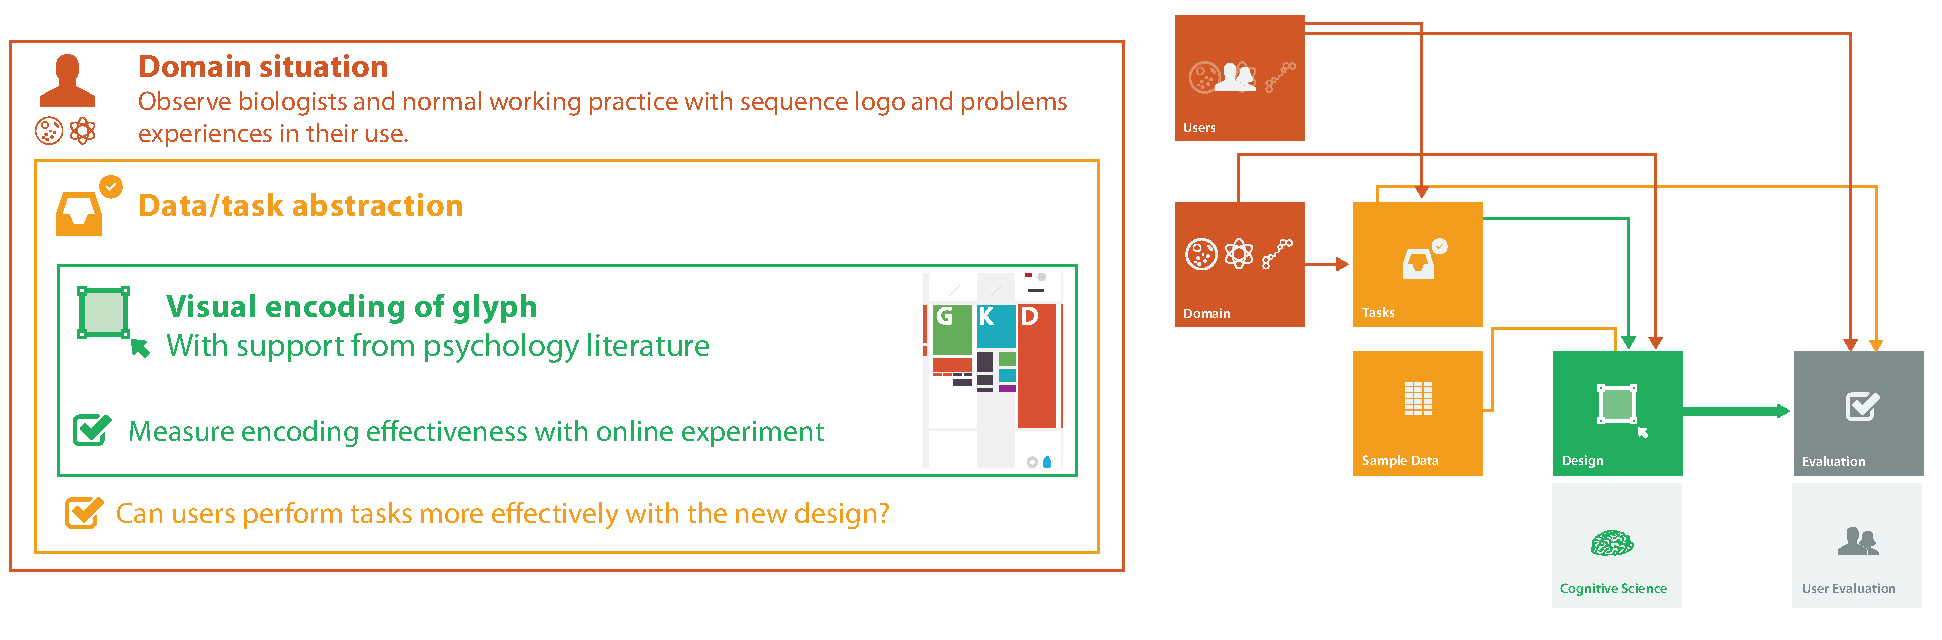
\includegraphics[width=\textwidth]{images/other_glyphs/sequence_process}
%\caption{}
%\label{fig:sequence_process}
%\end{figure}
%
%
%\item \textbf{Poetry visualization} in Section \ref{sec:poetry}, involved the creation of glyphs to support poetry scholars in their exploration of a poem and its features.
%This work involved close collaboration with a user community and involves a two-stage design process:
%
%\begin{enumerate}
%
%\item The first is the creation of a glyph design for poems that encompasses the semantic and phonetic information at each word, and shows semantic and phonetic connections across words and lines.
%This glyph design process was informed by Munzner's \emph{nested model} since no computation was used to inform the design process, and evaluation was carried via continuos but largely remote domain expert interaction; and
%
%\item The second piece of work extends on the first through provision of an overview or ``macro'' glyph to show how sounds progress within a poem. The design process follows the \emph{nested model for glyph design} approach through making use of computational approaches to generate statistics on the data which informed the glyph design process.
%To \emph{evaluate} the approach, we conducted semi-structured user interviews with domain experts.
%
%\end{enumerate}
%
%\item \textbf{File system visualization} in Section \ref{sec:file_system} involves the creation of glyphs to mark different event types in a file system.
%The \emph{design process} involved the formation of a theoretic concept to help in the creation of visually distinct glyphs. This involved the collection of benchmark measures to help construct the theory, and an evaluation of glyph designs derived from the application of the theory.
%These benchmark measures involved two types of measurement: human-centred; and machine-centred study.
%
%\end{enumerate}
\newpage
\section{Glyph-based Solutions for Biological Sequence Analysis}
\label{sec:sequence_logo}

%-------------------------------------------------------------------------
Advances in DNA sequencing technologies have turned a time consuming and expensive process into a quasi-mainstream commodity.
Next generation sequencing allows exploration of the blueprints of life in fascinating new ways, making the genome of thousands of species available to computational analysis.
Of particular interest to scientists is the detection of regions of genomes under selective pressure and to ascertain which regions of DNA, RNA and proteins are functionally and/or structurally important across species (\eg, the conserved regions of a protein in mice, human, rat, and horse).

Although our ability to process this data has increased, the methods used to visualize and report this conservation in scientific publications has not moved on in over 20 years.
This dominant method, named the ``sequence logo'' \cite{Schneider.Stephens1990,Schneider2002} is comprised of a series of letters stacked on top of each other.
It is reliance on these letters and their arrangement that cause perception problems \cite{biovis_redesign}. 
%
Here we introduce a new sequence logo design aimed at addressing their perception issues using design principles from Chapter \ref{chap:related_work}. 
Our approach is a three stage process, with a domain-expert always in the loop:

\begin{enumerate}
\item improving the current \emph{sequence logo} design to address perceptual issues caused by: a) use of letter size to represent value; and b) the arrangement of letters on the y-axis, which can make residues look more conserved than others based on the number of letters it is stacked upon;

\item adding \emph{glyphs} to annotate positions with chemical properties of particular residues to aid interpretation of the effect of alternations in different species for example; and

\item an evaluation of the redesigned sequence logo with both advanced and 'naive' sequence logo users to ascertain the benefits of the new design.
\end{enumerate}

\subsection{Background}

Transcription factors, as shown in Figures \ref{fig:binding} A and B are proteins with a central function; they can, with high specificity, recognize and bind to DNA regions, triggering transcription of DNA into RNA.
These DNA regions are known as transcription factor binding sites (TFBS) and their identification is essential to the reconstruction of transcriptional regulatory networks of cells.
As shown in Figure \ref{fig:binding} C, sequence comparison across organisms can be used to highlight areas of conservation to pinpoint unknown TFBS.
Low variability at some position $i$ generally points to a level of functional importance in that region of DNA or protein, pointing to selective pressure. 

\begin{figure}[h!]
\centering
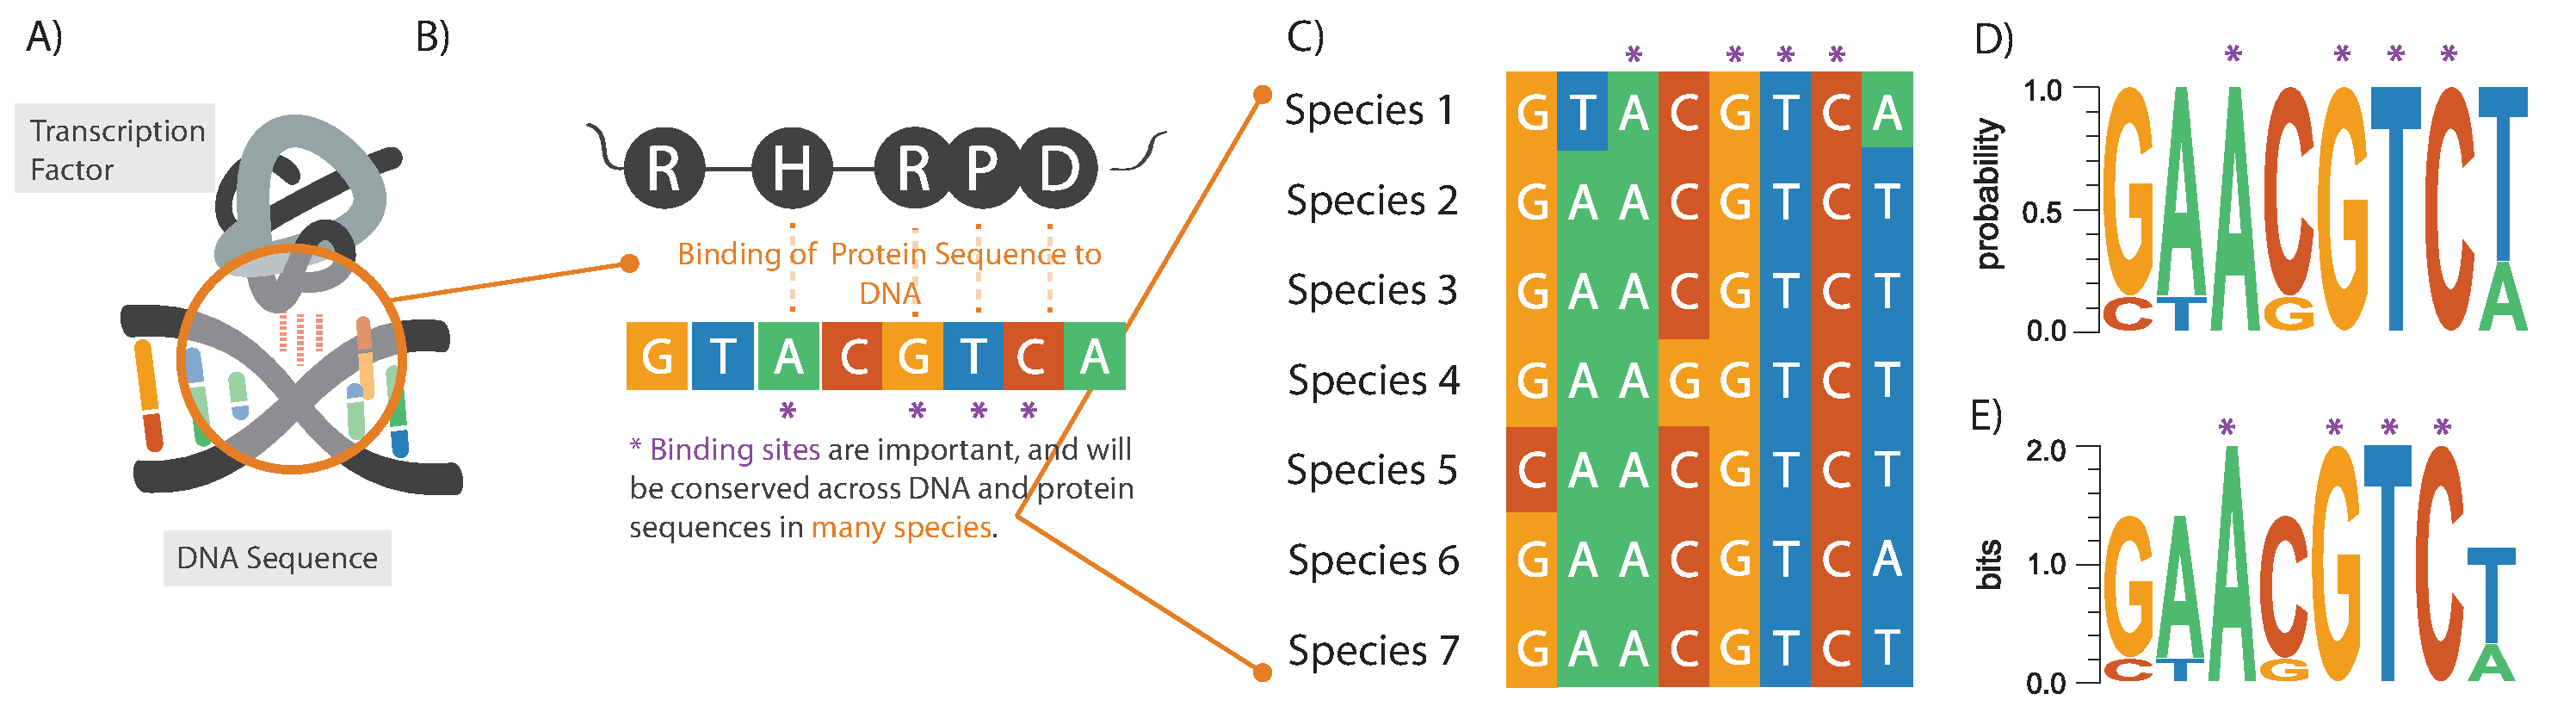
\includegraphics[width=\textwidth]{images/other_glyphs/sequence_logo/binding}
\caption{A) An abstraction of a transcription binding site where a protein binds to a region of DNA.
B) Certain residues, amino acids for the protein and DNA nucleotides for DNA are important in creating a bond between the DNA and protein to enable some function to occur (\eg, DNA repair).
C) The DNA of seven species is compared which shows a number of conserved regions where the DNA nucleotide is always the same (marked with a blue asterix). In a large matrix with many hundreds or thousands of sequences, this can be difficult to visualize.
D) Sequence logos provide a way of showing conserved regions. Probability based sequence logos assign the height of a letter in proportion to the number of times it appeared in that position.
E) Entropy-based sequence logos adjust the height of each letter based on the amount of ``surprise'' at each sequence rather than just the probability.}
\label{fig:binding}
\end{figure}

In order to visualize these binding sites, sequence logos were devised as a visualization technique to view a position weight matrix (PWM), which specifies for each position in a sequence the likelihood of observing a particular residue (DNA/RNA nucleotide or amino acid). From this matrix, a simple frequency-based sequence logo can be drawn by iterating through each position $i$ in the sequence (see Figure \ref{fig:binding} D). For each position, the height of each letter $a$ can be calculated as $p(a) \times R$ where $p(a)$ is the measured probability of $a$ occurring at position $i$, and $R$ is the maximum height at position $i$.

An alternative approach is to determine the maximum height at position $i$ by computing its ``information content'', a term derived from Claude Shannon's information theory\cite{Shannon1948}.
Information content represents the level of certainty at a specific position $i$ by measuring how much the probability distribution of the detected letters in that position deviates from a uniform distribution, where all valid letters have an equiprobable chance of occurring.
Given $s$ valid letters, $a_j, j=1, 2, \ldots, s$, in an alphabet $\mathbb{Z}$ and their probability distribution function, $p(a_j)$, the level of uncertainty can be defined by the following entropy measure:
\[
H(\mathbb{Z}) = -\sum_{j=1}^s p(a_j) log_2 p(a_j)
\]

\noindent where the logarithm is base two, and the unit for the uncertainty $H$ is ``bit''.
For an equiprobable distribution, $p(a_j) = 1/s$ for all letters in the alphabet $\mathbb{Z}$.
The above entropy measure yields the maximum uncertainty (commonly referred to as the maximum entropy), $H_{max}(s) = log_2 (s)$.

\noindent For example, for twenty-one amino acids, we have $H_{max}(21) = 4.39$ bits, and for 4 types of nucleic acids, $H_{max}(4) = 2$ bits.

Since it is unlikely that there is an equiprobable distribution of letters at each position $i$, the actual uncertainty is usually less than $H_{max}$.
Therefore the difference between the maximum uncertainty and the measured uncertainty can be defined as the certainty, which is visually encoded as the total height $R_i$ for all letters at position $i$.

As shown in Figure \ref{fig:binding} E, a high stack indicates a high level of certainty with a strong preference for one or at most two nucleotides.
A low stack implies a low level of certainty with many possibilities.
The idea behind this visual design is that the highly conserved positions ``pop out'' more due to their greater height.

%\subsection{Related Work}
%
%There have been a few attempts to redesign the sequence logo in the past, with most having focused on modifying how such letters are positioned on the y-axis with Kullback Leibler \cite{kullback1951}, position-specific scoring matrix (PSSM) \cite{fujii2004}, and berry logos \cite{berry2006,berrylogo}. These in part can alleviate some of the perception issues with the sequence logo, though all continue to use letters to represent size apart from LogoBar by Perez \emph{et al} \cite{perez2006logobar}. We extend on the work by Perez through support for DNA/RNA sequences, glyphs, an evaluation and a web-based implementation.

%-------------------------------------------------------------------------

\subsection{Design Process}

Our design process involved the application of design principles from Chapter \ref{chap:related_work} to help in the creation of a new sequence logo that circumvented frailties in the old design.
This process involved the following steps where there were both feedforward and feedback steps:

\begin{enumerate}
\item\textbf{Review of original design with domain experts}; 
\item\textbf{Presentation of design options};
\item\textbf{Implementation}; and
\item\textbf{Evaluation using an online user survey}.
\end{enumerate}

\begin{figure}[t!]
\centering
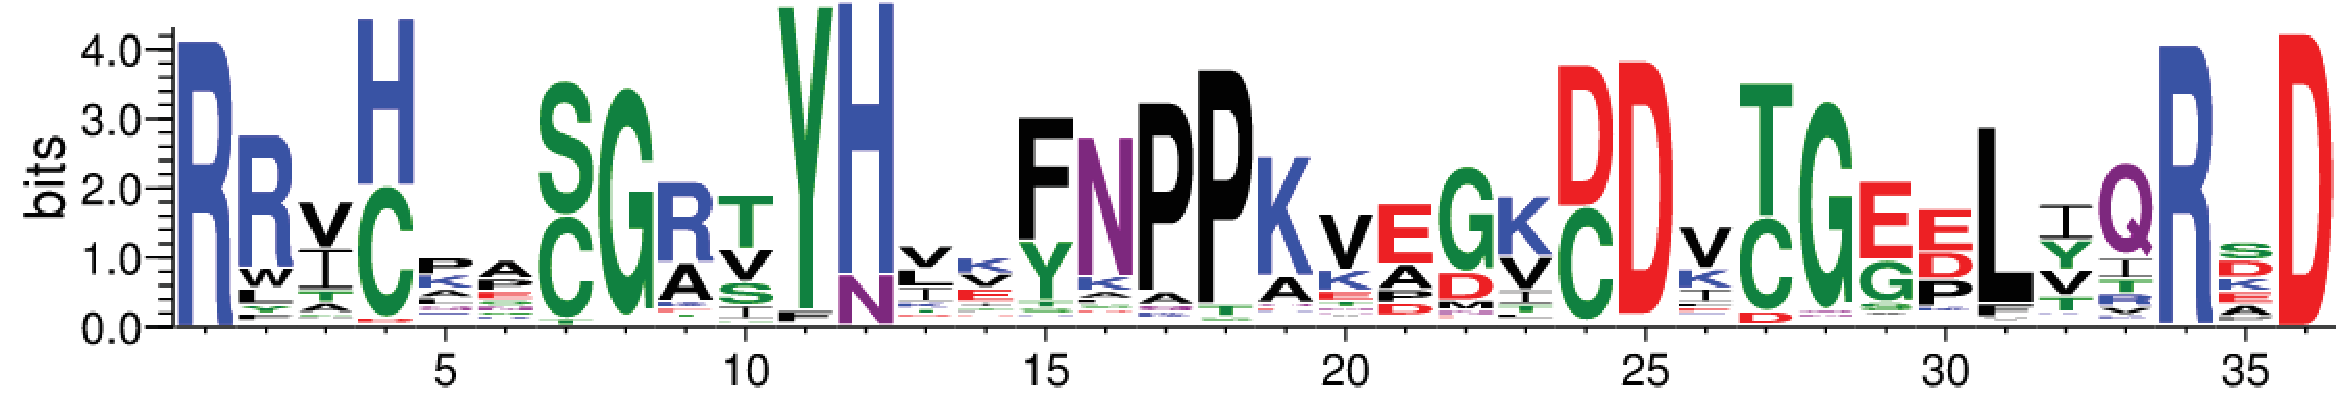
\includegraphics[width=\textwidth]{images/other_glyphs/sequence_logo/old-sequence-logo}
\caption{A traditional sequence logo generated using WebLogo \url{http://weblogo.threeplusone.com} from the BioVis redesign contest data \cite{biovis_redesign} showing the conserved regions across 1809 protein sequences.}
\label{fig:sequence_logo_design_teaser}
\end{figure}

\textbf{Review of original design with domain experts}. The weaknesses of the original sequence logo may be summarized as follows: 
\begin{enumerate}
\item \emph{Using letter size to show value} --- letters have an undesirable property in that they are of differing densities. We have quantified this effect (see Figure \ref{fig:letter-area}) and found that and \emph{R}, \emph{H} and \emph{W} take up to about three times as much ink as \emph{I} ,\emph{J} or \emph{L} for example.
When used for space filling, this ultimately leads to perception issues as denser letters will be more visible.
Use of letters also means that when there many variants at a given position, letters become ``squashed'' so it is often impossible to read them;

\begin{figure}[b!]
\centering
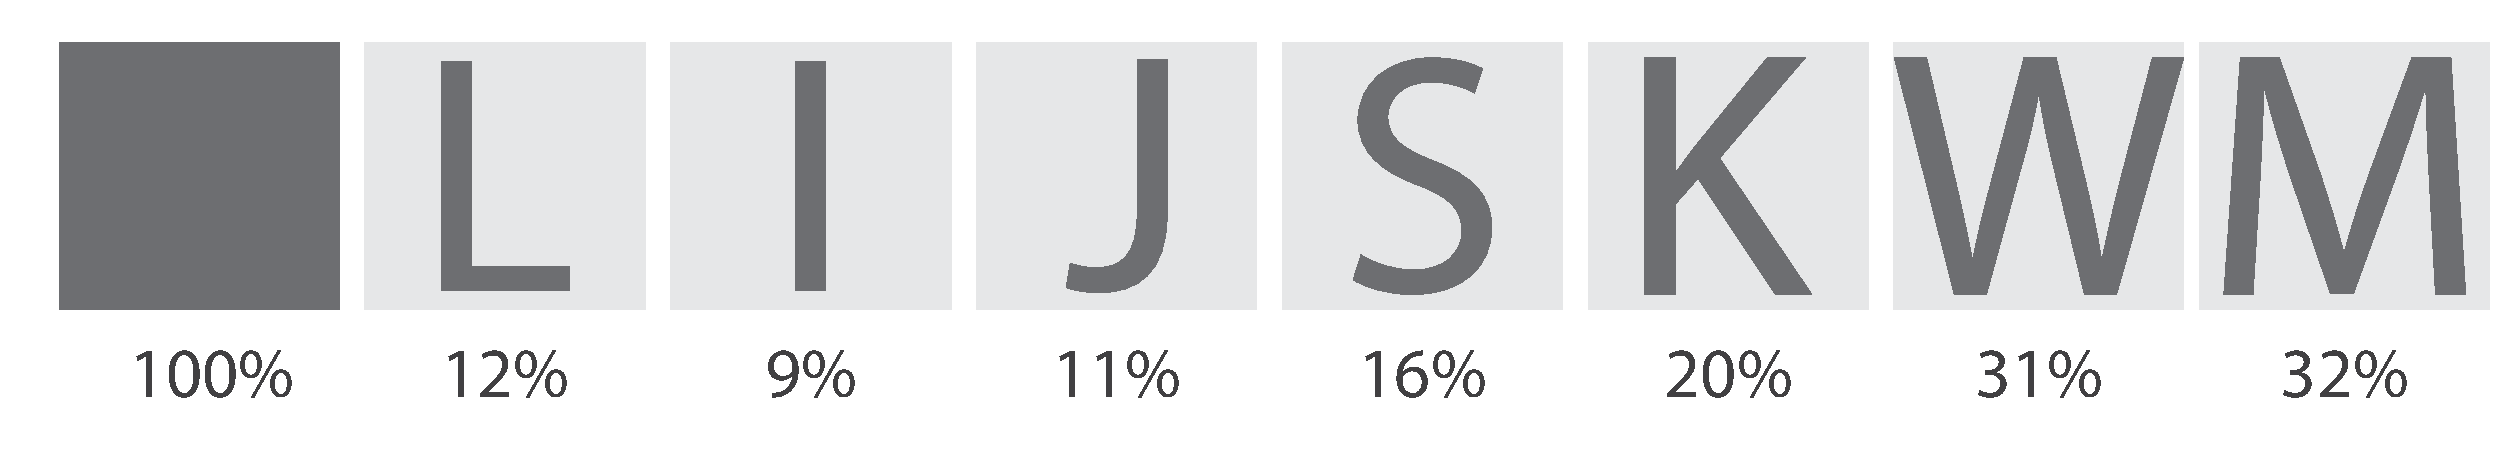
\includegraphics[width=.6\textwidth]{images/other_glyphs/sequence_logo/space}
\caption{The amount of ink used in a letter can influence the perceived `weight' of the letter. \emph{W} and \emph{M} take up three times as much ink as \emph{I}, \emph{J}, and \emph{L}, and twice as much as \emph{S}.}
\label{fig:letter-area}
\end{figure}

\item \emph{Placement of the most dominant letter on top of the less dominant letters, leading to possible misinterpretation of the size of a letter depending on where it is placed on the y axis} --- this is particularly evident in Figure \ref{fig:sequence_logo_design_teaser} at positions 2 and 4 where we may compare heights between `R' (Arginine) and `H' (Histidine).
In Figure \ref{fig:sequence_logo_design_teaser}, `H' is positioned higher in the chart due to the letters below it.
This gives the impression that the conservation of `H' at position 4 is greater than the conservation of `R' at position 2. In reality, `R' is more conserved at position 2.
\end{enumerate}

\textbf{Presentation of design options}. Any new design should retain the core principles of the original sequence logo to ease uptake of a new representation, whilst subtly overcoming its perception issues.
Initially, this design process involved the creation of a number of options shown in Figure \ref{fig:sequence_design_options} to improve on the current letter-based approach. 
These design options were filtered to just one following feedback from domain experts as well as consideration of research presented in Chapter \ref{chap:related_work}, in particular the research by Cleveland and McGill \cite{cleveland1984graphical}, and Heer and Bostock \cite{heer2010crowdsourcing}.

\begin{figure}[t!]
\centering
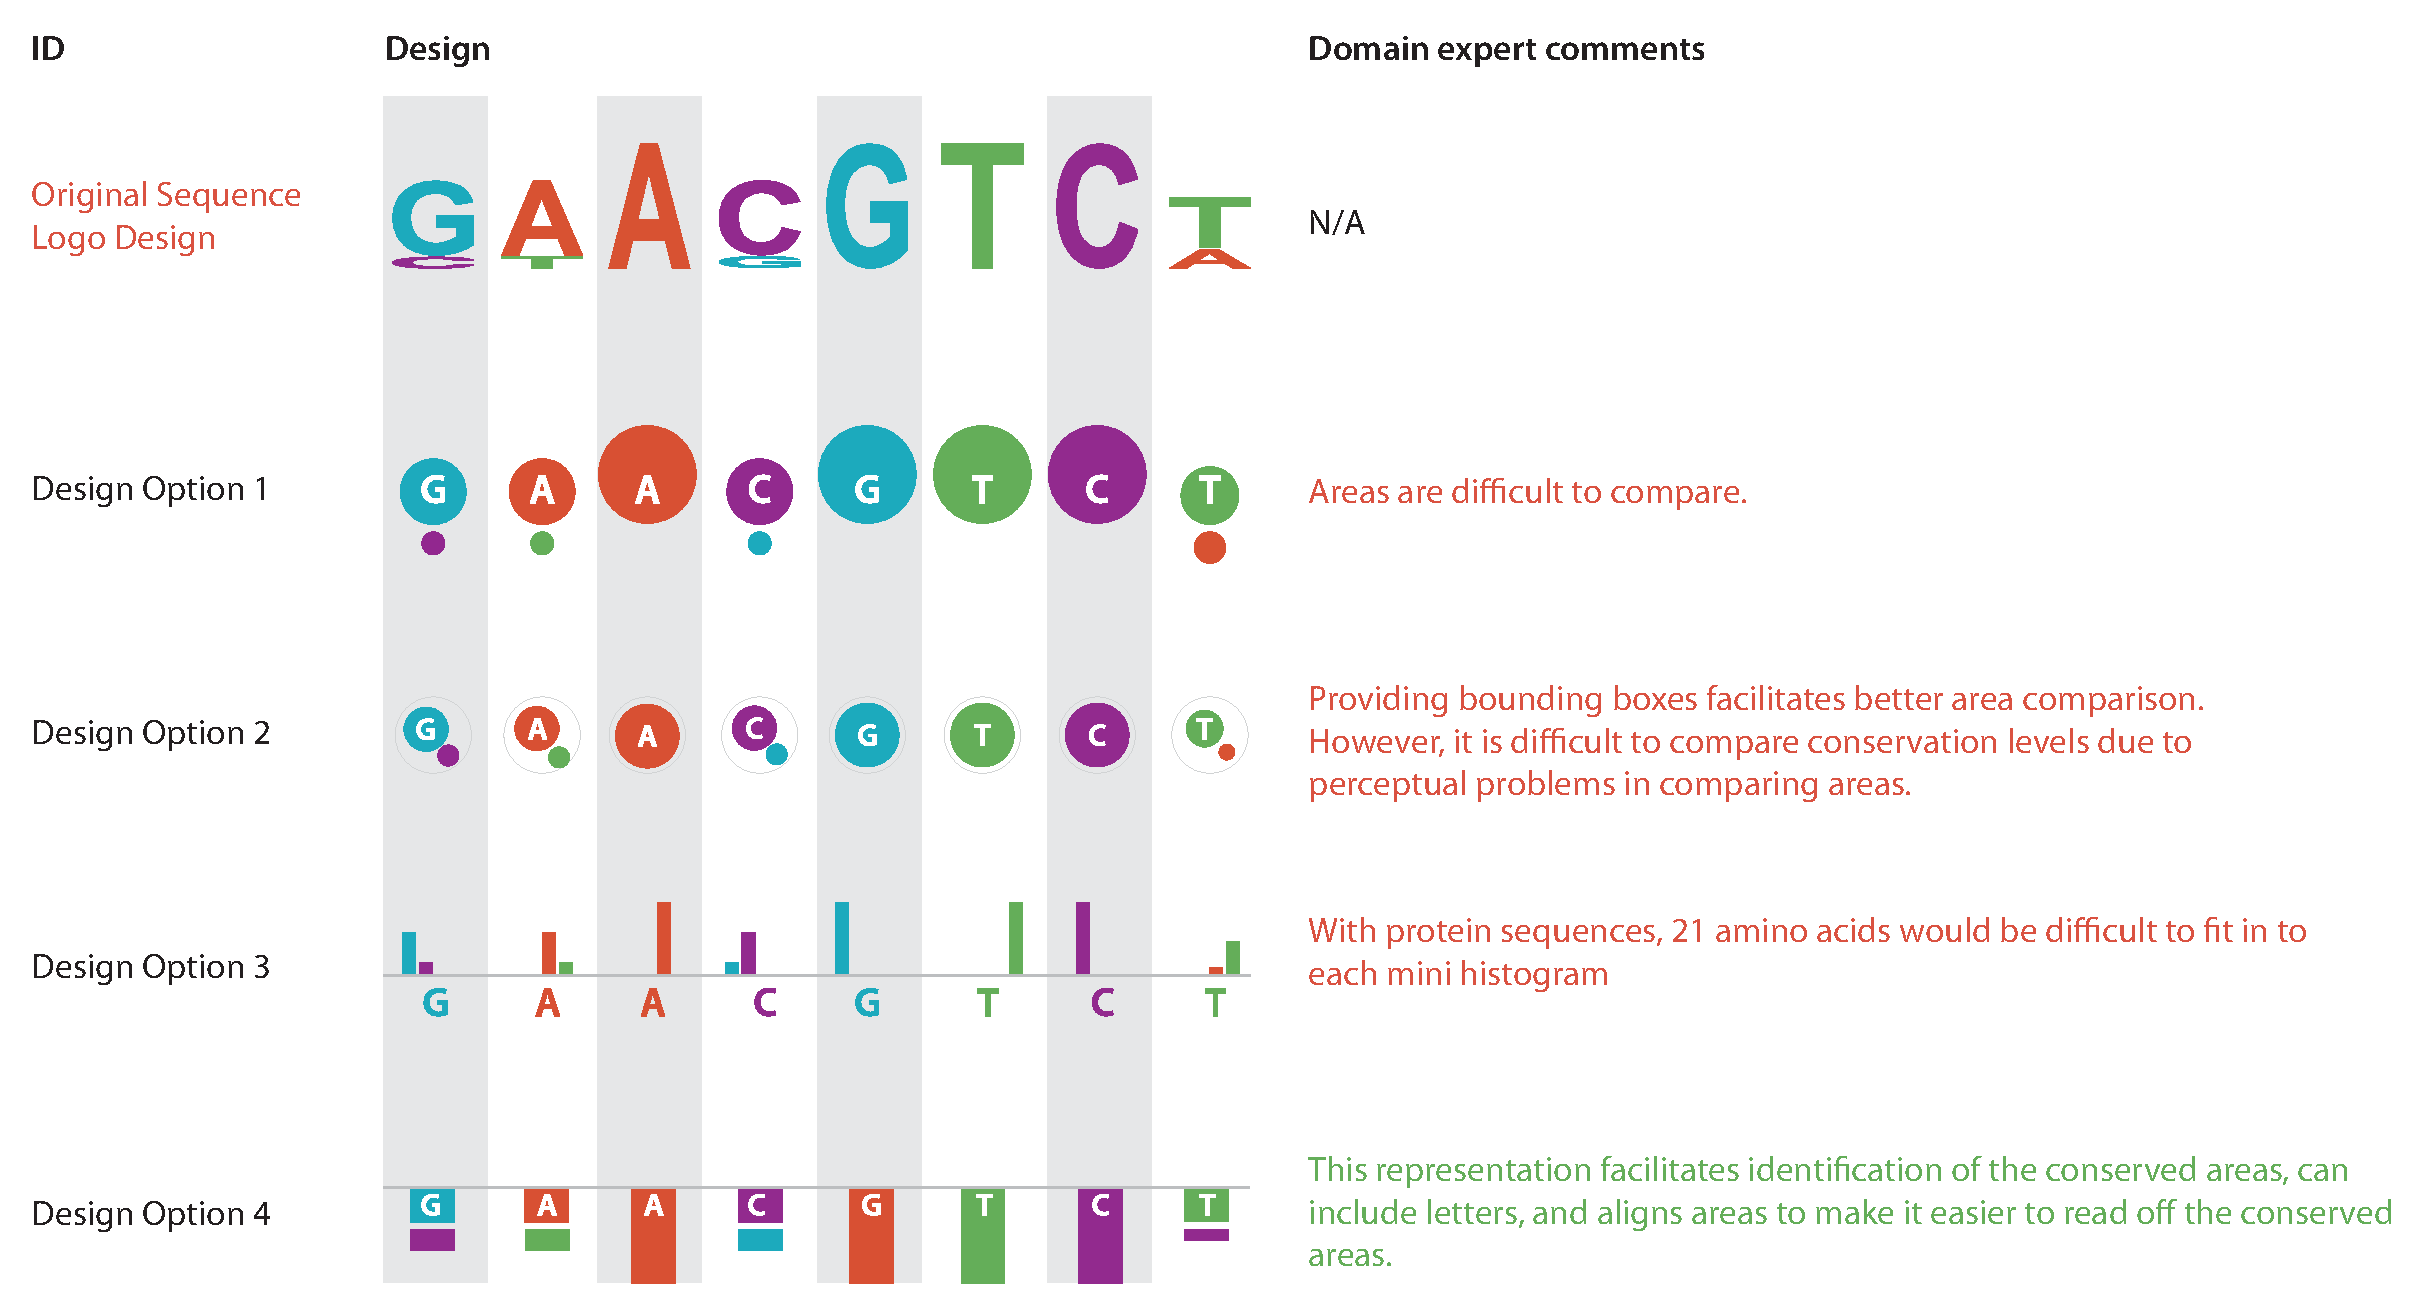
\includegraphics[width=\textwidth]{images/other_glyphs/sequence_logo/design_options}
\caption{A number of design options and reasons for excluding them based on research by Cleveland and McGill \cite{cleveland1984graphical} and Heer and Bostock \cite{heer2010crowdsourcing}.}
\label{fig:sequence_design_options}
\end{figure}

Our final design, shown in Figure \ref{fig:sequence-logo-design} uses filled bars to represent size in place of the letters.
The top `residues' (amino acids or nucleotides) are positioned at the top or bottom of the plot so that the conserved sequence can be read more easily than in the original logo.
The colours of the bars are a function of the type of amino acid.
However, these colours are not fixed and may be altered depending on how the user prefers to visually group residues.

\begin{figure}[b!]
\centering
\includegraphics[width=.75\textwidth]{images/other_glyphs/sequence_logo/sequence-logo-design}
\caption{Redesign of the sequence logo layout from the original (left) to the new version. Bars may be aligned to the top or bottom. At each position, residues are displayed in order of their conservation.}
\label{fig:sequence-logo-design}
\end{figure}

Amino acid residue side-chain charge and hydrophobicity strongly affect protein folding and its final 3D conformation, so any significant change in those qualities may result in a significant functional change.
By providing a visual aid to remind users of those dimensions, we offer the opportunity for enhanced interpretation.
Additionally, we experiment with another glyph-based approach, named ``Gestalt Lines'' \cite{brandes2013gestaltlines} to provide an additional indication of variance at a position. 

\begin{figure}[t!]
\centering
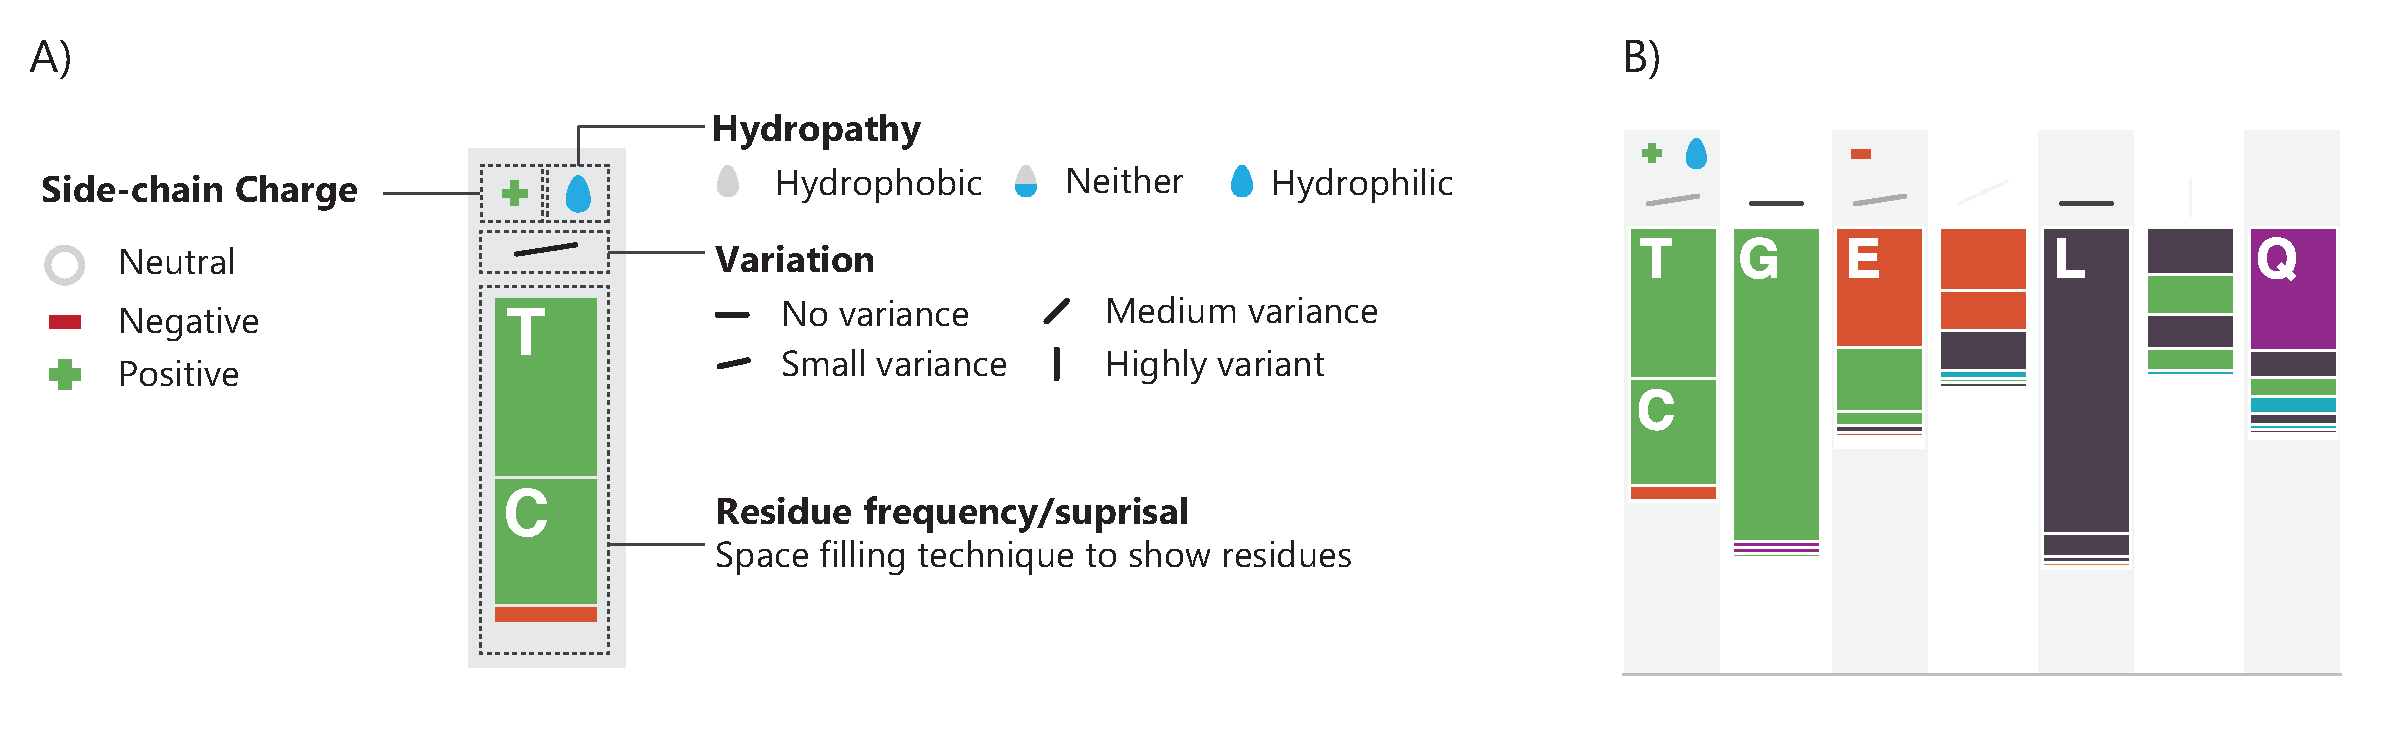
\includegraphics[width=\textwidth]{images/other_glyphs/sequence_logo/glyphs}
\caption{A) Overall glyph design has a number of regions to support glyph placement for interpretation, such as hydropathy, and side-chain charge.
Variation is also shown via ``GestaltLines'' \cite{brandes2013gestaltlines}.
B) A glyph is shown at a position in the sequence to form the overall sequence logo.}
\label{fig:glyphs}
\end{figure}

The glyphs provide an overall indication of any dominating characteristics of the amino acids present at a given position.
These glyphs, in context with the redesigned sequence logo are shown in Figure \ref{fig:glyphs}.
Glyphs for hydropathy and side-chain charge are only present in amino acid sequence logos. 

%-------------------------------------------------------------------------

\subsection{Evaluation}

\begin{figure}[b!]
\centering
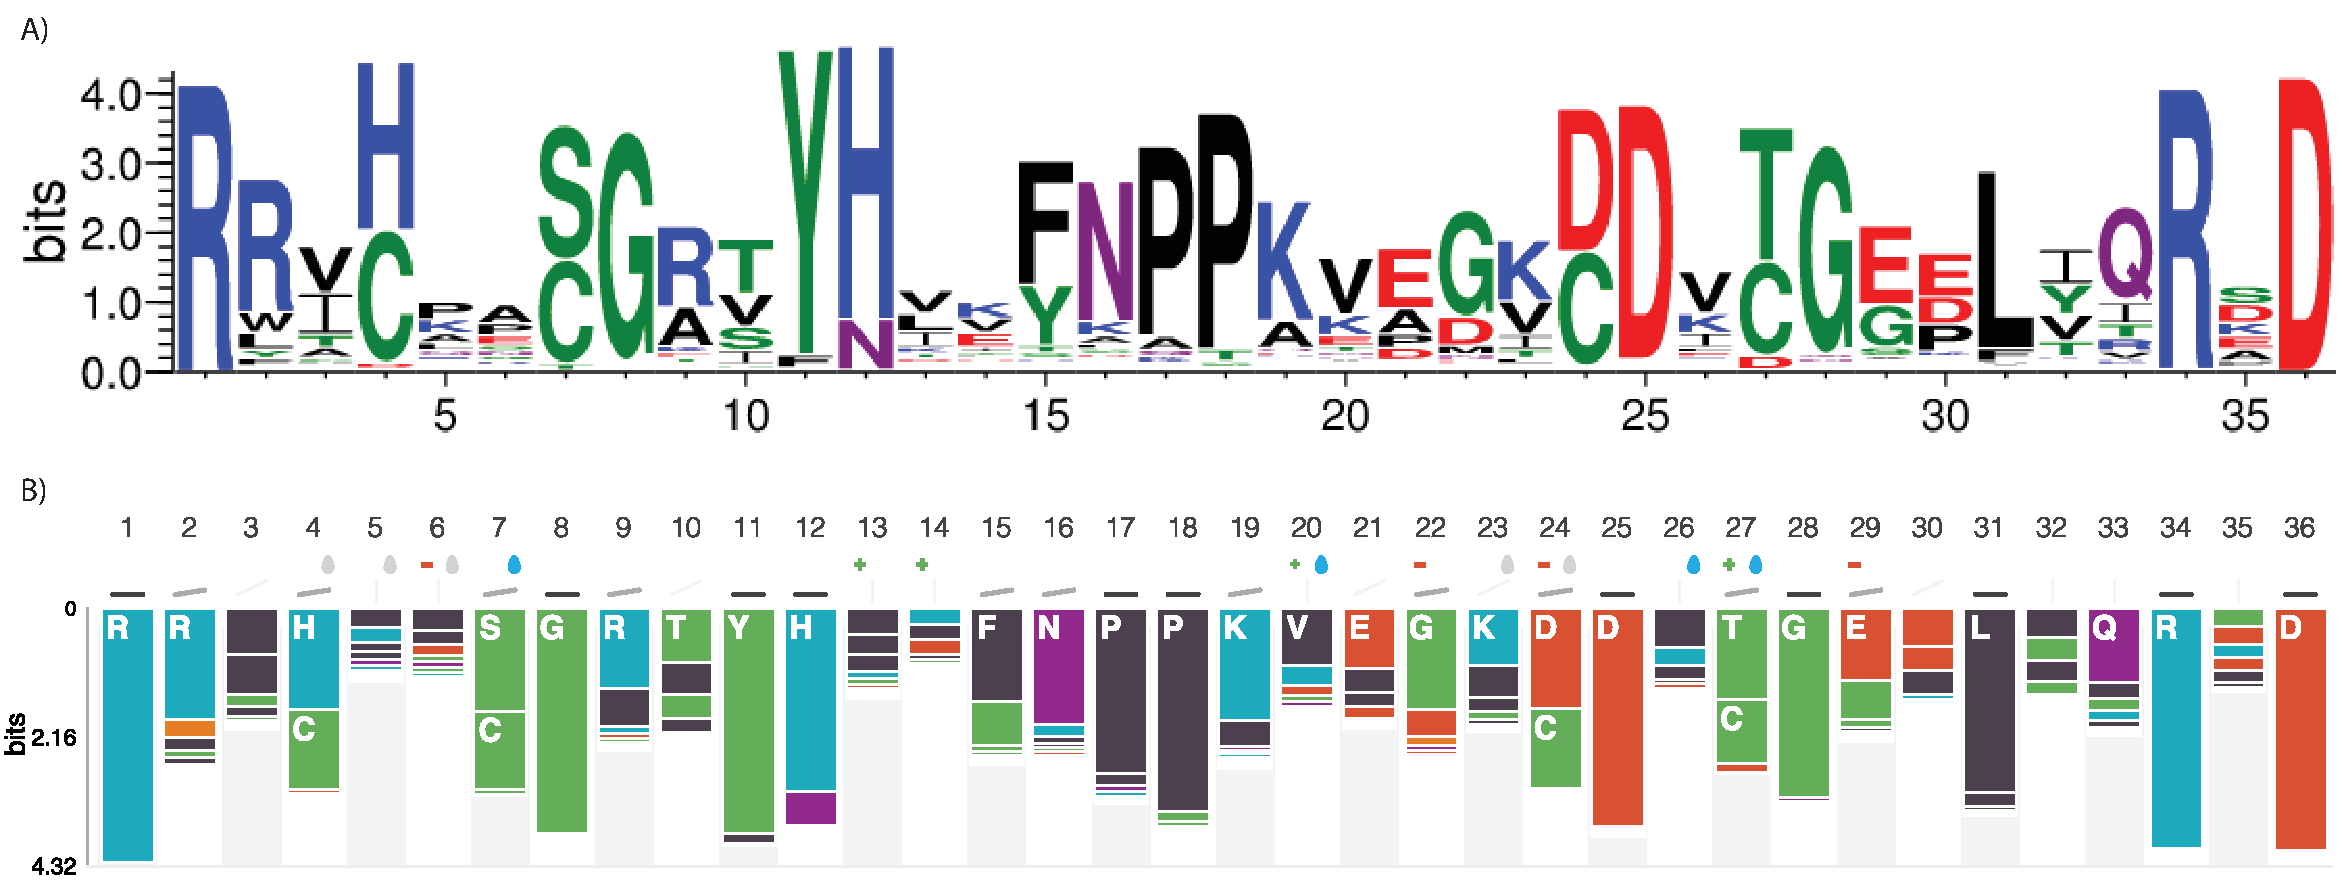
\includegraphics[width=\textwidth]{images/other_glyphs/sequence_logo/old_and_new_design}
\caption{A) Traditional sequence logo representation. B) New sequence logo representation.}
\label{fig:old_and_new}
\end{figure}

In order to assess if our changes helped biologists in their interpretation of sequence logos, we devised a survey focused on evaluating the ability to compare the size of letters in the old version of the sequence logo (see Figure \ref{fig:old_and_new} A) and the new version (Figure \ref{fig:old_and_new} B). We used the same data to create the two versions of the sequence logo and asked participants to determine which letter between two was the largest.
Our hypothesis, as stated earlier, is that it is harder to compare letters than blocks. Forty-one scientists (fifteen bioinformaticians, twenty-three biologists and three computer scientists) with varying levels of familiarity with sequence logos, took part in the survey.

\begin{figure}[t!]
\centering
\includegraphics[width=\textwidth]{images/other_glyphs/sequence_logo/evaluation}
\caption{Evaluation responses showing the ability to discriminate between conservation levels in the two designs of the sequence logo, old/original and new.}
\label{fig:evaluation}
\end{figure}

Figure \ref{fig:evaluation} shows survey results (upper part) and test images (lower part).
In three out of the four questions given to users, a higher number of correct answers were recorded with the new sequence logo.
The gain was significant for questions two and three, with up to twice as many correct answers with the new representation. The exception was in question four, where there was a small (8\%) advantage gained by using the original version.
The greater density of `G' over `L' may have lead to more people choosing correctly by chance, explaining the observation. More thorough experimentation would be needed to validate this hypothesis however.

The feedback from users regarding the glyphs was also largely positive with: 80\% of respondents agreeing that showing hydropathy was useful; 83\% agreeing that showing side-chain charge was useful; and 59\% indicating that the variance glyph using GestaltLines was useful.
The feedback led to the removal of the ``GestaltLines'' from the entropy-based height encoding since the level of variance can be adequately determined using bar height alone.
For frequency-based height encoding, ``GestaltLines'' are more useful since all bars are the same height.

The approval of our redesign was also measured with users asked to give their preference between Figures \ref{fig:sequence_logo_design_teaser} A and B. 95\% of respondents said that they preferred the new representation over the original, citing amongst others, `cleanliness' and `clarity' as major factors in their decision.
%
%\subsection{Contributions}
%We have presented a new design for the sequence logo that incorporates glyph-based techniques to aid interpretation. 
%We have also provided an implementation of this new logo available at \url{https://github.com/ISA-tools/SequenceLogoVis} that can be incorporated into the workflows of scientists for interactive use or inclusion in publications.
%Our usability tests showed that users generally found consensus sequence reading tasks easier with the new sequence logo. Users, on the whole, agreed that the new representation did a better job of improving the display of salient information.
%
%This work was published as a short paper and presented at EuroVis 2015 in a paper entitled \emph{Redesigning the Sequence Logo with Glyph-based Approaches to Aid Interpretation} \cite{CGF:maguire14-sp}.


\newpage
\section{Glyph-based Solutions for Poetry Visualization}
\label{sec:poetry}

\subsection{Background}
Poems to some may be seen as nothing more than a sequence of words.
To poets however, they are a complex system with many links between words (\eg, rhyming patterns, and alliteration), different interpretations, and various ways of reading the same text (there is no indication of exact timing as in music for instance).
A technique called ``close reading'' aims to explore the complexity of such a system through hours of literary analysis devoted to a poem of interest. 
Such readings investigate many aspects of a poem including: 
\begin{enumerate}
	\item formal information (\eg, lines, and stanzas);
	\vspace{-2mm}
	\item phonetic information (\eg, meter, intonation, and timing);
	\vspace{-2mm}
	\item semantic information (\eg, genres, words, repetition, and sentiment); and
	\vspace{-2mm}
	\item context-driven information (\eg, geographical location, historical period, and political affiliation).
\end{enumerate}

\begin{figure}[b!]
\centering
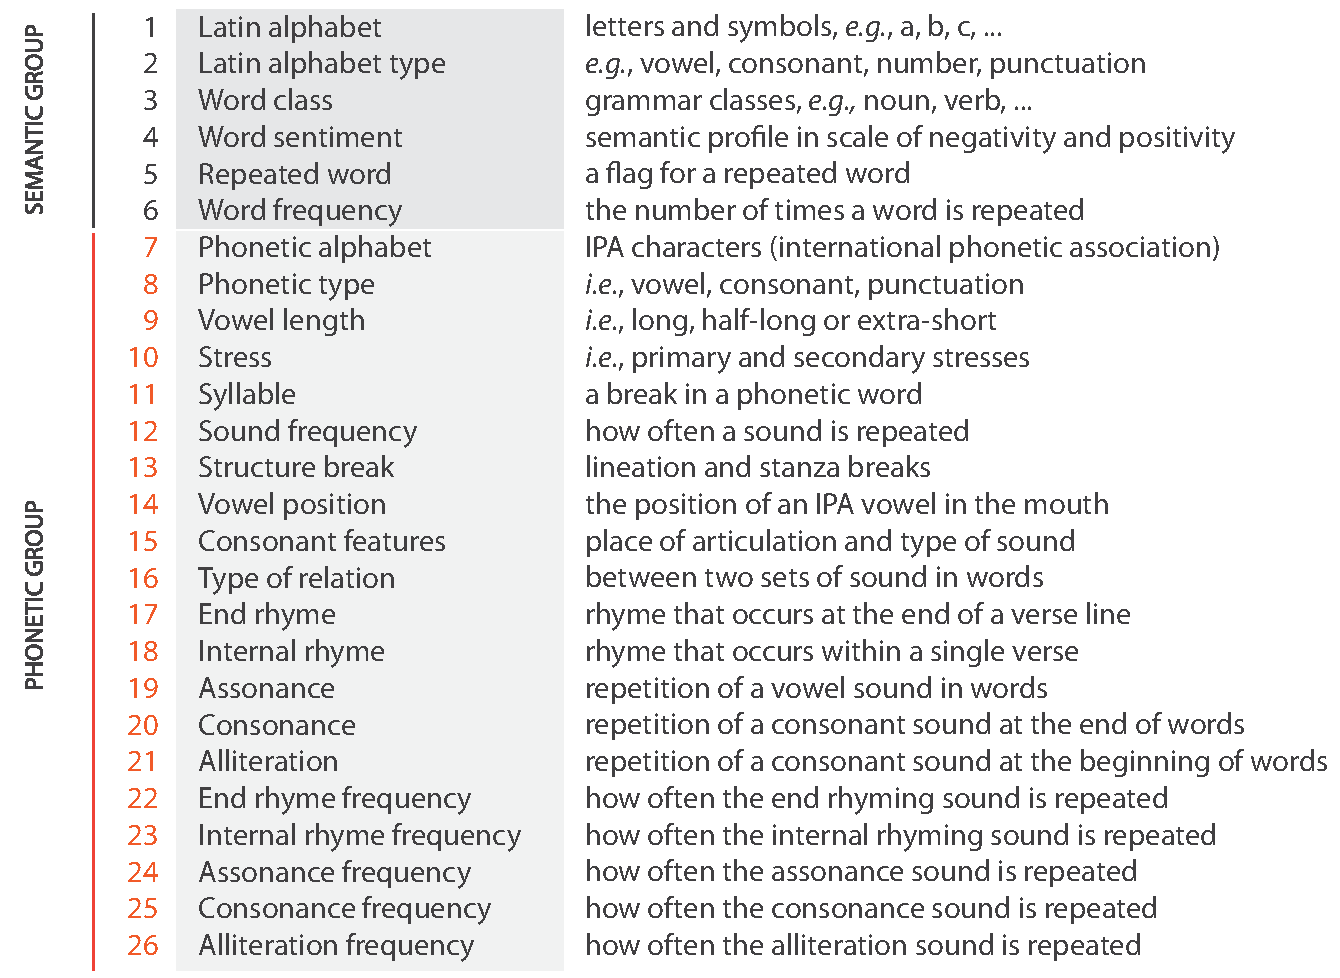
\includegraphics[width=\textwidth]{images/other_glyphs/poem_glyph_vars}
\caption{The six semantic and twenty phonetic variables representing a poem identified from investigatory discussions with domain experts.}
\label{fig:poem_glyph_vars}
\end{figure}


From investigatory discussions with the two poetry scholars from the University of Utah and a linguist from the University of Oxford, thirty-three variables were initially identified, although only twenty-six were deemed useful for poetry scholars.
These two set of variables shown in Figure \ref{fig:poem_glyph_vars} are there to help poetry scholars answer questions such as: 
\begin{enumerate}
	\item Which of the words in the poem rhyme with each other?
	\vspace{-2mm}
	\item What is the rhyming pattern in the poem?
	\vspace{-2mm}
	\item How much sound turbulence is in the poem (changes in the type of sound made through pronunciation of a word)?
	\vspace{-2mm}
	\item How many of the vowels are rounded vowels?
	\vspace{-2mm}
	\item Where are the caesurae (line pauses) in the poem?
	\vspace{-2mm}
	\item How many of the caesurae are masculine caesuras (pause following a stressed syllable)? and
	\vspace{-2mm}
	\item How many of the caesurae are feminine caesurae (pause following an unstressed syllable)?
\end{enumerate}

In all, fifty two tasks were identified.
Analysis of these tasks showed that not all variables were required all of the time. 
Classes of task required different variables.
What this meant in terms of visual design is that variables may have different levels of importance depending on the task at hand. 
This is in contrast to the work in the previous chapters where there was invariance in the importance of variables.

%The first piece of work investigates the use of knowledge from previous chapters to create a rule-based approach to help systematise glyph design. 
%Such a rule-based framework would allow for \emph{controlled} user-defined mappings of the twenty-six poem variables to visual channels.
The first piece of work investigates the creation of a visualization of poetry data facilitated by glyphs.
It also looks at the design of a mini-glyph required to show how sounds are produced in the mouth.

The second piece of work extends on the first through creation of static and animated overview glyphs (termed macro glyphs) for each line of a poem to show vowel sound changes/turbulence over time.
We use statistics to help creation of static and animated glyph designs.
This is followed by an evaluation of a selection of designs by four domain experts.

A web application named \emph{Poem Viewer} \url{http://www.ovii.org/PoemVis/} brings together both contributions for use by poetry scholars.

%although seven were removed due to not being suitable to English text (classification between pulmonic (sounds created by air-pressure from the lungs) or non-pulmonic consonants (ejective, implosive or click)), 

\subsection{Glyph Design for Poetry Visualization}

\subsubsection{Design Process}

Given the twenty six poetic variables defined in Figure \ref{fig:poem_glyph_vars}, the aim was to create a glyph design that would support their encoding and facilitate some fluidity in how the glyphs were constructed to support different types of task.
Our design process followed the ``nested model'' approach from Munzner \cite{munzner2009nested}.
This model was adopted due to its support for agile development with user engagement and inclusion of feedback at every stage of the design process.
Close interaction with domain experts was important in this work due to the poetry domain being relatively untouched by visualization research in the past.
Here we describe the design of the: 
\begin{enumerate}
\item \textbf{poem component glyph} that represents the features of each component, this being a word or punctuation mark for example in a poem.
Each glyph can connect to other glyphs to show relations between components of a poem (\eg, rhyming patterns and alliteration); and 
\item \textbf{vowel position ``mini glyph''} that shows the properties of vowel sounds and how they are produced.
\end{enumerate}

\textbf{Poem component glyph}. The overall glyph design needs to support encoding of the twenty-six poetic variables shown in Figure \ref{fig:poem_glyph_vars}.
The categorisation in Figure \ref{fig:poem_glyph_vars} divides the twenty-six variables in to semantic and phonetic groups.
Within each of these groups, further sub divisions can be made, these are:

\begin{enumerate}
\item\textbf{Phonetic}:
\begin{itemize}
\item \textbf{Phonetic Relations} between sounds and how they are pronounced \eg, rhyme, end rhyme (line endings that sound the same), alliteration, assonance (repeating vowel sounds), and consonance (repeating consonant sounds). 
%This region uses of line colour to represent the different types of relation, and line thickness to represent frequency;
\item \textbf{Phonetic Features} showing how the sound is made for vowels and/or consonants \eg, whether the sound is made from the back of the mouth with the tongue up (closed) or down (open) as shown in Figure \ref{fig:poem_glyph_design} B.
%This region makes use of pictograms like those shown in Figure \ref{fig:poem_glyph_design} B or symbol shape and colour to represent this data;
\item \textbf{Phonetic Units and Attributes} displays the phonetic alphabet, the type (vowel, consonant or punctuation), vowel length, stress (primary or secondary), syllable breaks, sound frequency, and structure break (new line);
\end{itemize}
\item\textbf{Semantic}:
\begin{itemize}
\item \textbf{Word Units and Attributes} displays the word, the type of each component within that word (vowel, consonant, or punctuation), the type of the word (\eg, noun, verb, adjective, adverb, or unknown), and the word sentiment; and
\item \textbf{Semantic Relations} between words of particular type or repetition of some word.
\end{itemize}
\end{enumerate}

A poem component can be a word or punctuation which may or may not have \emph{phonetic features}, \emph{phonetic units and attributes}, and \emph{word units and attributes}.
Each component can be linked together by their \emph{phonetic relations} (alliteration, assonance, consonance, or rhyme), or \emph{semantic relations} (repeated word, frequency, or sentiment).
Each poem component will be assigned a glyph representing it, alongside connections representing the relations between one or more poem components. 
This arrangement of glyphs creates the overall poem visualization.

Each of the sub divisions described above may be thought of as a region of the glyph.
These regions should be organised consistently to facilitate comparison between each glyph in a poem.
Furthermore, consistency will make it easier for users to perform visual search owing to the expectation of finding particular pieces of information in distinct areas of a glyph.
Two regions, \emph{phonetic relations}, and \emph{semantic relations}, require the representation of relational information.

\begin{figure}[b!]
\centering
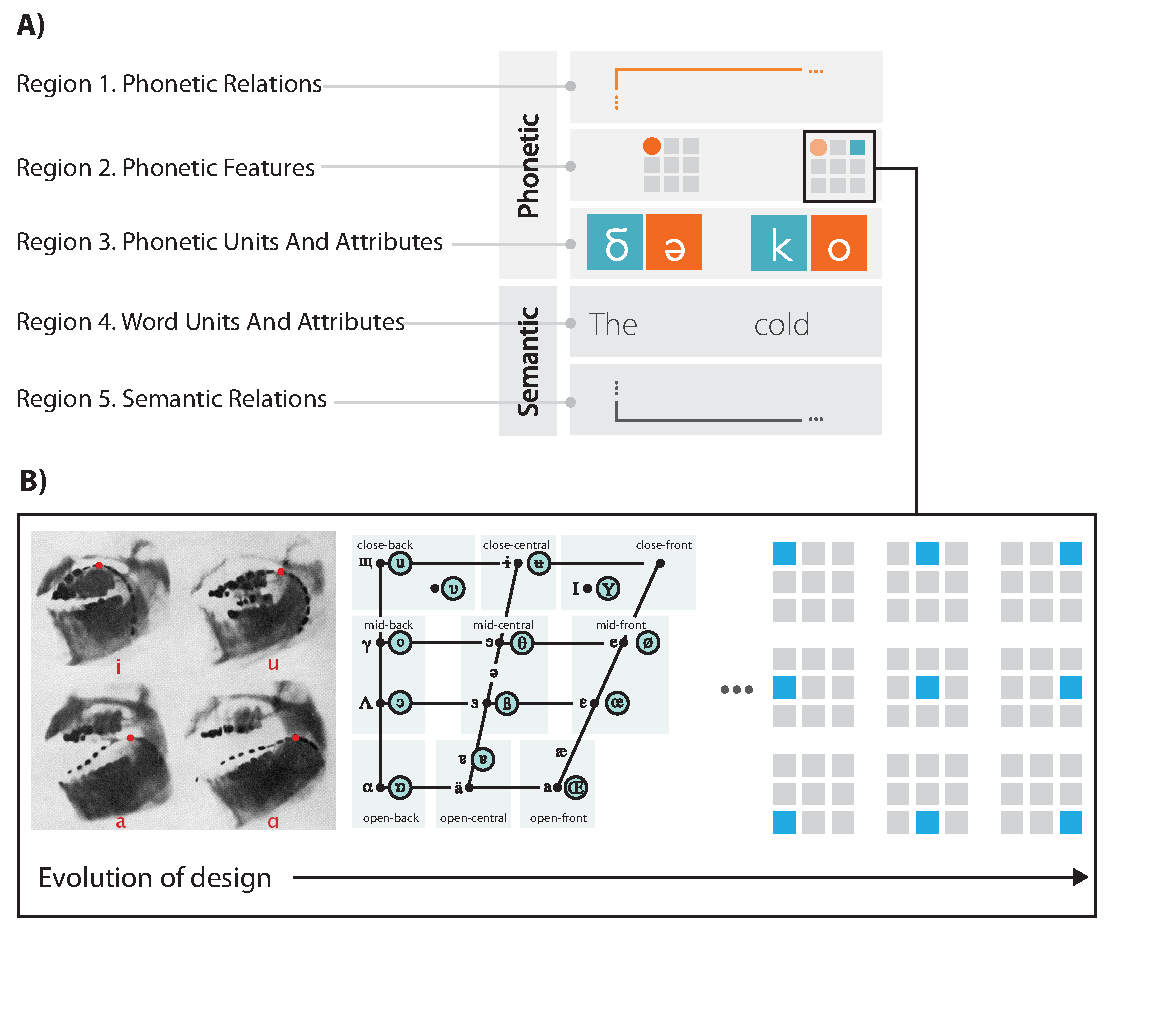
\includegraphics[width=.75\textwidth]{images/other_glyphs/poem_glyph_design}
\caption{A) The glyph design encompasses five regions to support semantic and phonetic variables listed in Figure \ref{fig:poem_glyph_vars}.
B) Evolution from the X-Ray scans of the mouth when pronouncing different vowel sounds, to the 5x7 IPA vowel chart, and finally to the 3x3 grid showing how the final sound is constructed by the different components of the mouth involved in speech.}
\label{fig:poem_glyph_design}
\end{figure}

The final arrangement of regions is shown in Figure \ref{fig:poem_glyph_design} and is largely driven by the phonetic/semantic divide.
Additionally, phonetic and semantic relation mappings were purposefully placed on opposite ends of the glyph to avoid line overlap. 
\emph{Phonetic units and attributes} were placed directly above the \emph{word units and attributes} since both were closely related and associating a word with a particular sound is important.
 
Due to users having changing needs, the type of data within some regions can be changed.
Additionally, the poetic to visual channel mappings can also be modified by users.
Appropriate mappings, or visual channels that are suitable for particular poetic variables, are automatically suggested to users via a ``rule-based mapping''  approach \cite{CGF:Abd2013a}.
This approach is inspired by the ``artificial assistant'' from Mackinlay \etal \cite{mackinlay2007show}, and informed by research presented in Chapters \ref{chap:related_work} and \ref{chap:glyph-tax}.


\begin{figure}[t!]
\centering
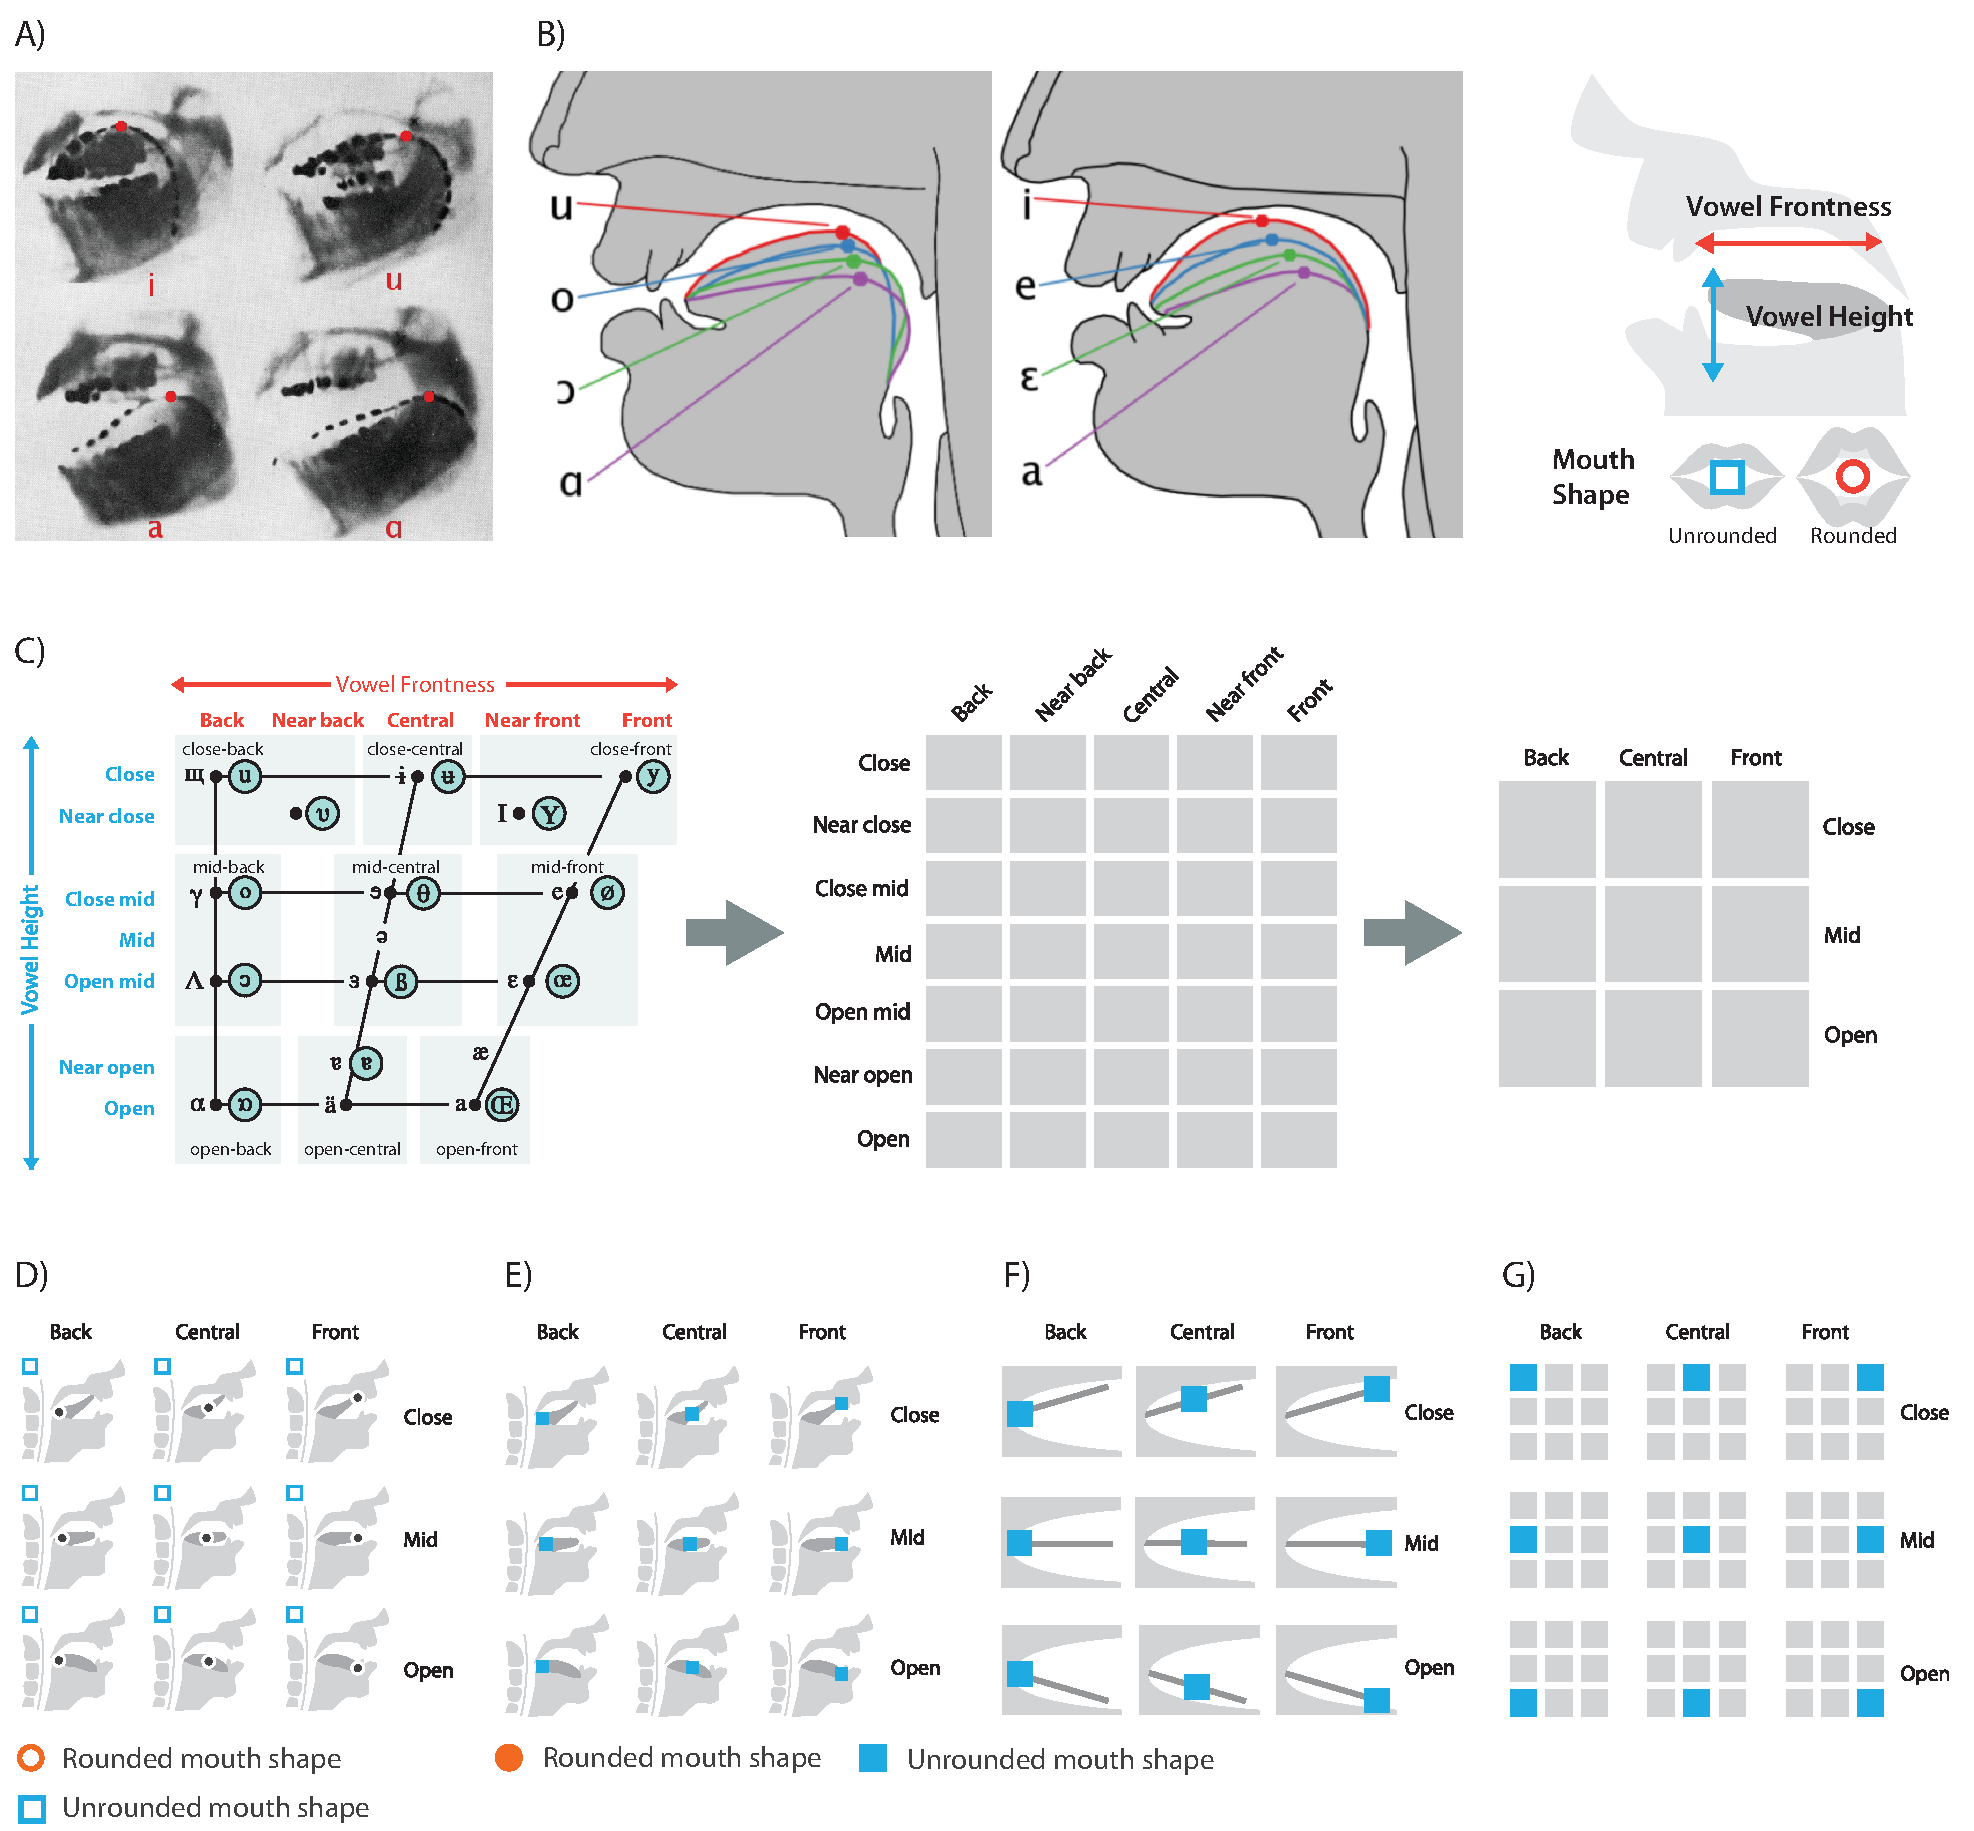
\includegraphics[width=\textwidth]{images/other_glyphs/poem-glyph-design-progression}
\caption{A) X-Ray scan from Jones \cite{jones1972outline} indicating the role of particular muscles in pronouncing certain vowels along with (some) marked up cross sections of a mouth and where vowel sounds originate.
Sound origin is shown with red marks that vary by height (vowel height) and distance from the back of the throat (vowel frontness).
B) Back (left) and front (right) vowel positions from Jones \cite{jones1972outline}.
C) The International Phonetic Alphabet (IPA) vowel chart \cite{ipa1999} arranges vowel sounds by the vowel height and vowel frontness properties that define those sounds in a 5x7 grid.
Through interactions with domain experts, it was found that this 5x7 matrix could be simplified to a 3x3 representation.
D) A first evolution of the design used a very metaphoric representation of the mouth, similar to those in \emph{B} and represent each of the positions from the 3x3 matrix achieved in \emph{C}.
The mouth is flipped since left was easier for users to interpret as the back due to how the glyphs were read from left to right.
Mouth shape is encoded by a shape in the top left of the mini glyph with a square with a blue stroke for unrounded, and an ellipse with an orange stroke for unrounded.
E) An extension of \emph{D} where mouth shape is encoded directly into the vowel frontness indicator as a square for unrounded and circle for rounded, with the addition of colour to provide further distinctiveness.
F) An abstraction on the first representation in \emph{C} that aimed to simplify the design for use in environments with lower resolutions. The line represents the tongue position.
G) The final 3x3 grid using coloured squares or circles at the position representing a vowel sound.}
\label{fig:poem_glyph_design_progression}
\end{figure}


\textbf{Vowel position ``mini glyph'' design}. In addition to the overall glyph design, a further design was devised to represent how a particular sound is constructed.
This ``mini glyph'', whose design process is summarised in Figure \ref{fig:poem_glyph_design} B, occupies the \emph{phonetic features} region in Figure \ref{fig:poem_glyph_design} A.
Each sound can be thought of as a particular configuration of specific muscles in the mouth.
This configuration includes the tongue position (vowel height), the shape of the mouth (rounded or unrounded), and the location in the mouth a particular sound originated (vowel frontness).
Figure \ref{fig:poem_glyph_design_progression} A shows a cross section of a mouth along with the different tongue positions (vowel height) and where in the mouth a sound originated using a red dot (vowel frontness).
Figure \ref{fig:poem_glyph_design_progression} B shows an abstract view of different vowel sounds and the configurations of vowel height and frontness that make these sounds possible.

The remaining components of Figure \ref{fig:poem_glyph_design_progression} show how the final glyph design came about and the design iterations made in chronological order from the initial abstraction step in Figure \ref{fig:poem_glyph_design_progression} C to each of the design options shown in Figure \ref{fig:poem_glyph_design_progression} D - G.
Figure \ref{fig:poem_glyph_design_progression} C starts with the IPA vowel chart \cite{ipa1999} that provides an organisation of the different vowel sounds by their vowel height and frontness parameters.
The chart may be represented by a 5x7 matrix, however this would be sparse since not all thirty-five positions would be used.
Following interactions with the domain experts, it was advised that this could be simplified to a 3x3 representation.

This 3x3 grid provided the general configurations of vowel height and frontness that needed to be represented by the mini glyph.
Further design iterations from Figure \ref{fig:poem_glyph_design_progression} D to G investigated the numerous ways glyphs could be represent to represent each configuration. 
Figure \ref{fig:poem_glyph_design_progression} D started with the mouth representation seen in Figure \ref{fig:poem_glyph_design_progression} B.
The hope was that a more metaphoric representation would make it easier for users to identify where sounds were coming from.
The tongue angle varies to reflect vowel height.
The position of the ellipse on the tongue represents the vowel frontness.
Progressing from this design, Figure \ref{fig:poem_glyph_design_progression} E encoded mouth shape directly on the vowel frontness indicator, using colour to provide increased differentiability.
Although the domain experts liked the design, the glyphs were difficult to interpret at lower resolutions, therefore we devised the design in Figure \ref{fig:poem_glyph_design_progression} F.
This kept the mouth metaphor in place, but made it more abstract so that more space could be afforded to the visual elements encoding information.
Again, users sometimes found it difficult to see differences between glyphs at the lower resolutions.
The final design, shown in Figure \ref{fig:poem_glyph_design_progression} G is able to represent all possible states through just using position, with colour and shape representing the mouth shape.
This design, although less metaphoric than the mouth could be interpreted even when the glyph was very small, so users preferred it.

\begin{figure}[t!]
\centering
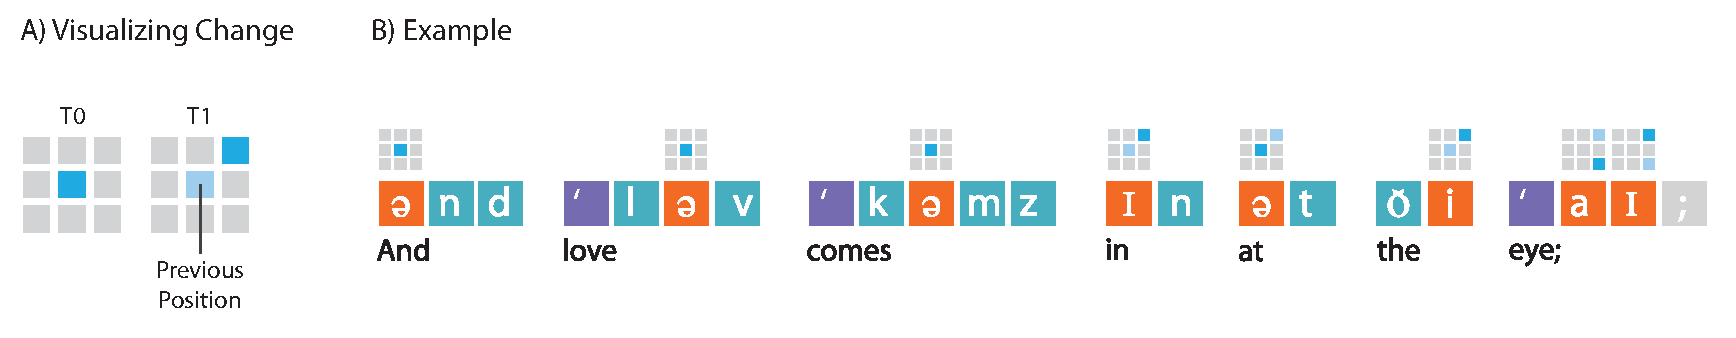
\includegraphics[width=\textwidth]{images/other_glyphs/poem_glyph_change}
\caption{A) The previous sound is maintained through making the shape representing that sound more transparent. B) In this poem, the changes can be seen in mouth position with the main sound being a front closed position (top right square) with an unrounded mouth.}
\label{fig:poem_glyph_change}
\end{figure}

Additionally, as shown in Figure \ref{fig:poem_glyph_change}, information about the previously encountered sound can be added to the glyph.
Showing the previous state allows users to see changes in the sound dynamics.
Smooth passages of sound should have relatively small changes, conversely, rough passages will have a greater number of changes.

\subsubsection{Evaluation}
The evaluation and design process were very much entwined in this work with frequent testing and feedback from domain experts that were part of a remote collaboration with poets from the University of Utah (Prof. Katherine Coles and Dr. Julie LeIn).


\subsection{Macro Glyphs for Poem Turbulence Summaries}

Following the initial poem glyph design, the poets wished to be able to gain an overview of how the sounds within a poem evolve/flow over time, a property known as the ``poem turbulence''.
From the previous work that presented a pictorial glyph design, it was not easy to follow the changes in sound over time.
The poetry scholars wished to observe patterns in sound changes to determine if certain types of poems have a particular type of ``turbulence pattern'', or within a poem are there patterns in sounds between lines?

While the first glyph design process used the nested model by Munzner \cite{munzner2009nested} as a framework to follow, this work followed a computational approach to glyph design as outlined in Chapter \ref{chap:strategies} with a user evaluation at the end.
In terms of process, this translates into the use of computational approaches to inform the design. Contrast this with the first piece of work where we relied heavily on user engagement to reach a final design.

\subsubsection{Macro Glyph Design Process}

Similar to Chapter \ref{chap:automacron}, this work proposes the use of ``macros'' (overview representations) to assemble many sound transitions in a single glyph.
This approach would solve the issue experienced by poets who wish to be able to see the overall flow of sounds across a line or poem as opposed to reading each pictogram for a vowel or consonant sound one by one.  
However, multiple macro design solutions are possible, all with advantages and disadvantages.
For this type of task, flow can be shown either statically or dynamically.
In this work we investigate a number of design options, both static and dynamic created using many of the techniques presented in the previous chapters to aid more systematised glyph design. 
The design options are evaluated with a number of poetry scholars to determine which performed better for tasks involved in understanding the sound patterns in poems.  

Of particular relevance to this thesis is the statistical approach taken in the design of the glyphs.
Thirty-five poems and other English texts (books and scientific publications) were analysed to determine the sounds and transitions present in the English language.
By analysing not just poems, a more accurate view of the transitions that occur in spoken English can be obtained.

\begin{figure}[t!]
\centering
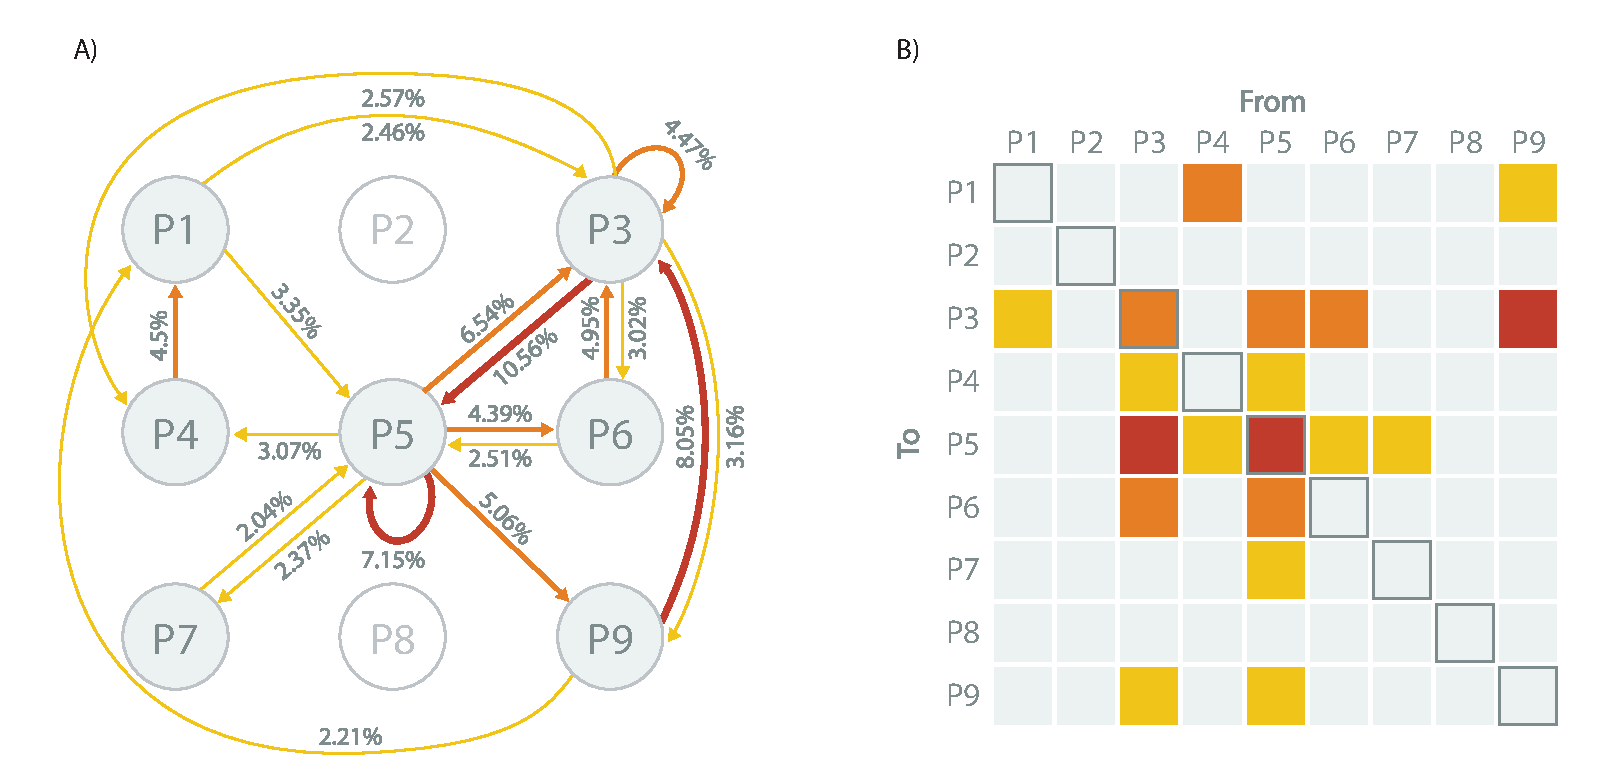
\includegraphics[width=\textwidth]{images/other_glyphs/macro_stats}
\caption{A) Graph showing vowel positions (see Figure \ref{fig:poem_glyph_design_progression} G) using nodes and the movements between each position using weighted edges as found in an analysis of 30 poems and English text.
The network shows that two positions are not used in the corpus of data observed.
B) Heat map showing the active areas in the network. 
Both A) and B) are coloured by the number of transitions from one position to another (grey is $f(p_a, p_b) = 0\%$, yellow ($0\%<f(p_a, p_b)< 4\%$), orange ($4\%<=f(p_a, p_b)<7\%$), and red ($f(p_a, p_b)>=7\%$)) where $p_a$ is the \emph{from} position and $p_b$ is the \emph{to} position.}
\label{fig:poem_statistics}
\end{figure}

The statistics gave us answers to the following questions: 
\begin{enumerate}
\item \emph{How many vowel phonemes (sounds that make words sound different from each other) were there per line?} The analysis showed that 84.3\% of lines contain $\leq$12 vowel phonemes and 22 is the maximum number of vowel phonemes;
\item \emph{How many movements were there in the frontness of the sound (back to front)?} The average difference in movement in movement is $\bar\mu=0.7709$ and the standard deviation $\sigma=0.7073$;
\item \emph{How many movements are there between open and closed tongue positions (termed vowel frontness)?} The average difference in movement in movement is $\bar\mu=0.8704$ and the standard deviation $\sigma=0.6699$; and 
\item How many transitions occurred between each position? The results to this are shown in Figure \ref{fig:poem_statistics}.
\end{enumerate}

The \textbf{static radial macro glyph} design benefitted from statistics 1) to 3). 
When the design process started, the number of spokes or lines representing each vowel phoneme was unknown. 
The seemingly obvious idea to make the number of lines dynamic would in fact make comparison between lines and positions more difficult. 
A small number of lines may result in the need for many macro glyphs to represent a line.
Conversely, a large number would result in a very densely packed macro glyph that was difficult to visually parse.

Statistic 1) showed that 84.3\% of lines contained twelve vowel phonemes or less, while the maximum number of vowel phonemes was twenty-two. 
Twelve fits well with the clock metaphor, and since the temporal aspect is important, familiarity with the clock would make such a glyph easier to interpret. 
The 15.7\% of lines that have more than twelve vowel phonemes would be accommodated through the use of two macro glyphs side by side. 
Alternatively, a twenty-four line glyph that could also fit the clock metaphor, could represent all of the vowel phonemes in lines, however 84.7\% of those lines would occupy less than half of the area of the glyph, and the more densely packed macro glyph would likely be more difficult to interpret.

Statistics 2) and 3) were used to inform which axis of the 3x3 vowel sound matrix (vowel frontness and height) would be mapped to a suitable visual channel. 
The variable with the greatest difference and deviation would be the ideal candidate for a mapping to position.
Unfortunately there was no outright winner, with vowel frontness having the larger standard deviation and vowel height having the largest average difference.
This led to a decision that proposed both options for evaluation by poets themselves to determine which mapping was more effective.
 
The \textbf{animated macro glyph} benefitted most from statistic 4). 
This statistic, summarised in Figures \ref{fig:poem_statistics} A and B, shows how many transitions there are between across the 3x3 matrix. 
Figure \ref{fig:poem_statistics} A shows a graph depicting all observed transitions with their probability of occurring.
Figure \ref{fig:poem_statistics} B presents a matrix-based representation of the graph view. 
It clearly indicates how only a small subset of all possible transitions between sounds are observed in the data (19/81), that positions two and eight have no observed uses, and finally that the greatest activity occurs around positions three and five.
Such analysis of the data would indicate that we can:
\begin{enumerate}

\item \emph{inform} the design process and implementation of the glyphs by exposing what transitions do and do not happen (from this analysis 19/81 transitions are observed in the data).
Therefore, instead of creating a glyph that needs to represent all possible transitions between nodes in the graph, many of these hypothetical transitions may be ignored, greatly simplifying the glyph design; and

\item enable the \emph{highlighting} of rare transitions and/or playing down the significance of frequent transitions if poets desired such functionality.

\end{enumerate}

The ability to inform the design process thanks to statistical analysis greatly simplified the design of the glyphs since the arcs between each position could be better arranged and decluttered.
For example, the knowledge of absence of transitions to/from positions two and eight made it possible to inform the animation algorithm to decrease the height of arcs running through positions one and three, and seven and nine. 
Additionally, where connections were uni-directional, the arcs could be less curved than they need to be when visualising a bi-directional connection. 

\begin{figure}[t!]
\centering
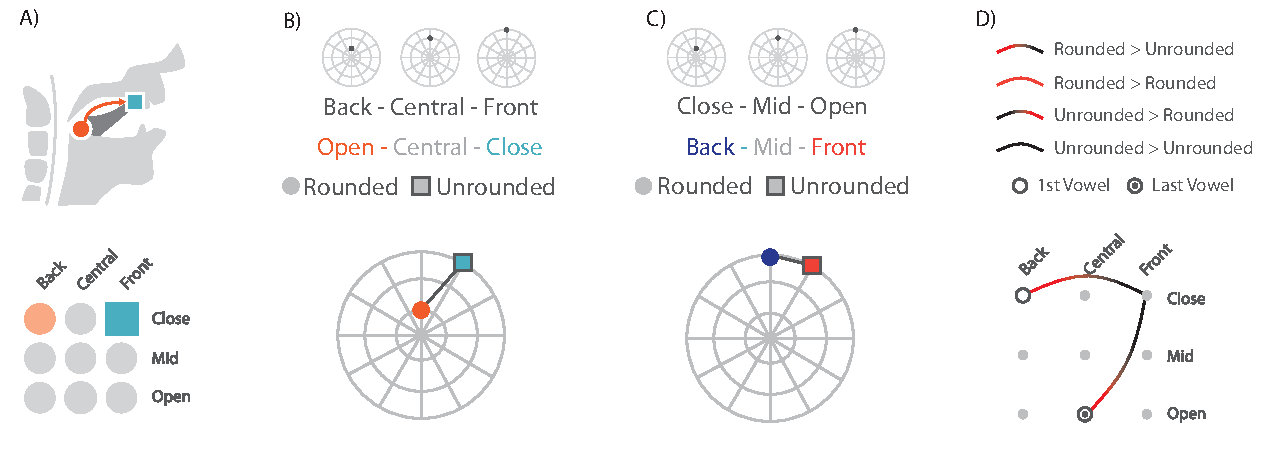
\includegraphics[width=\textwidth]{images/other_glyphs/poem_macro_design}
\caption{Four glyph representations showing how a particular sound is formed.
A) This is the original representation of sound movement.
B) A radial layout where time zero is at the top. This representation supports eleven sounds arranged temporally where the difference in distance from the inner to outer rings indicates the change in the sound origin (back to the front of the mouth).
C) An alternative radial layout where the position relates to the tongue being opened, in the middle, or closed.
D) An animated glyph design showing the flow between points in the 3x3 matrix using animation.
}
\label{fig:macro_glyph}
\end{figure}

Figure \ref{fig:macro_glyph} shows the resulting designs of the static radial macro glyphs and the overall schematic for the animated macro glyphs.
 

\begin{figure}[t!]
\centering
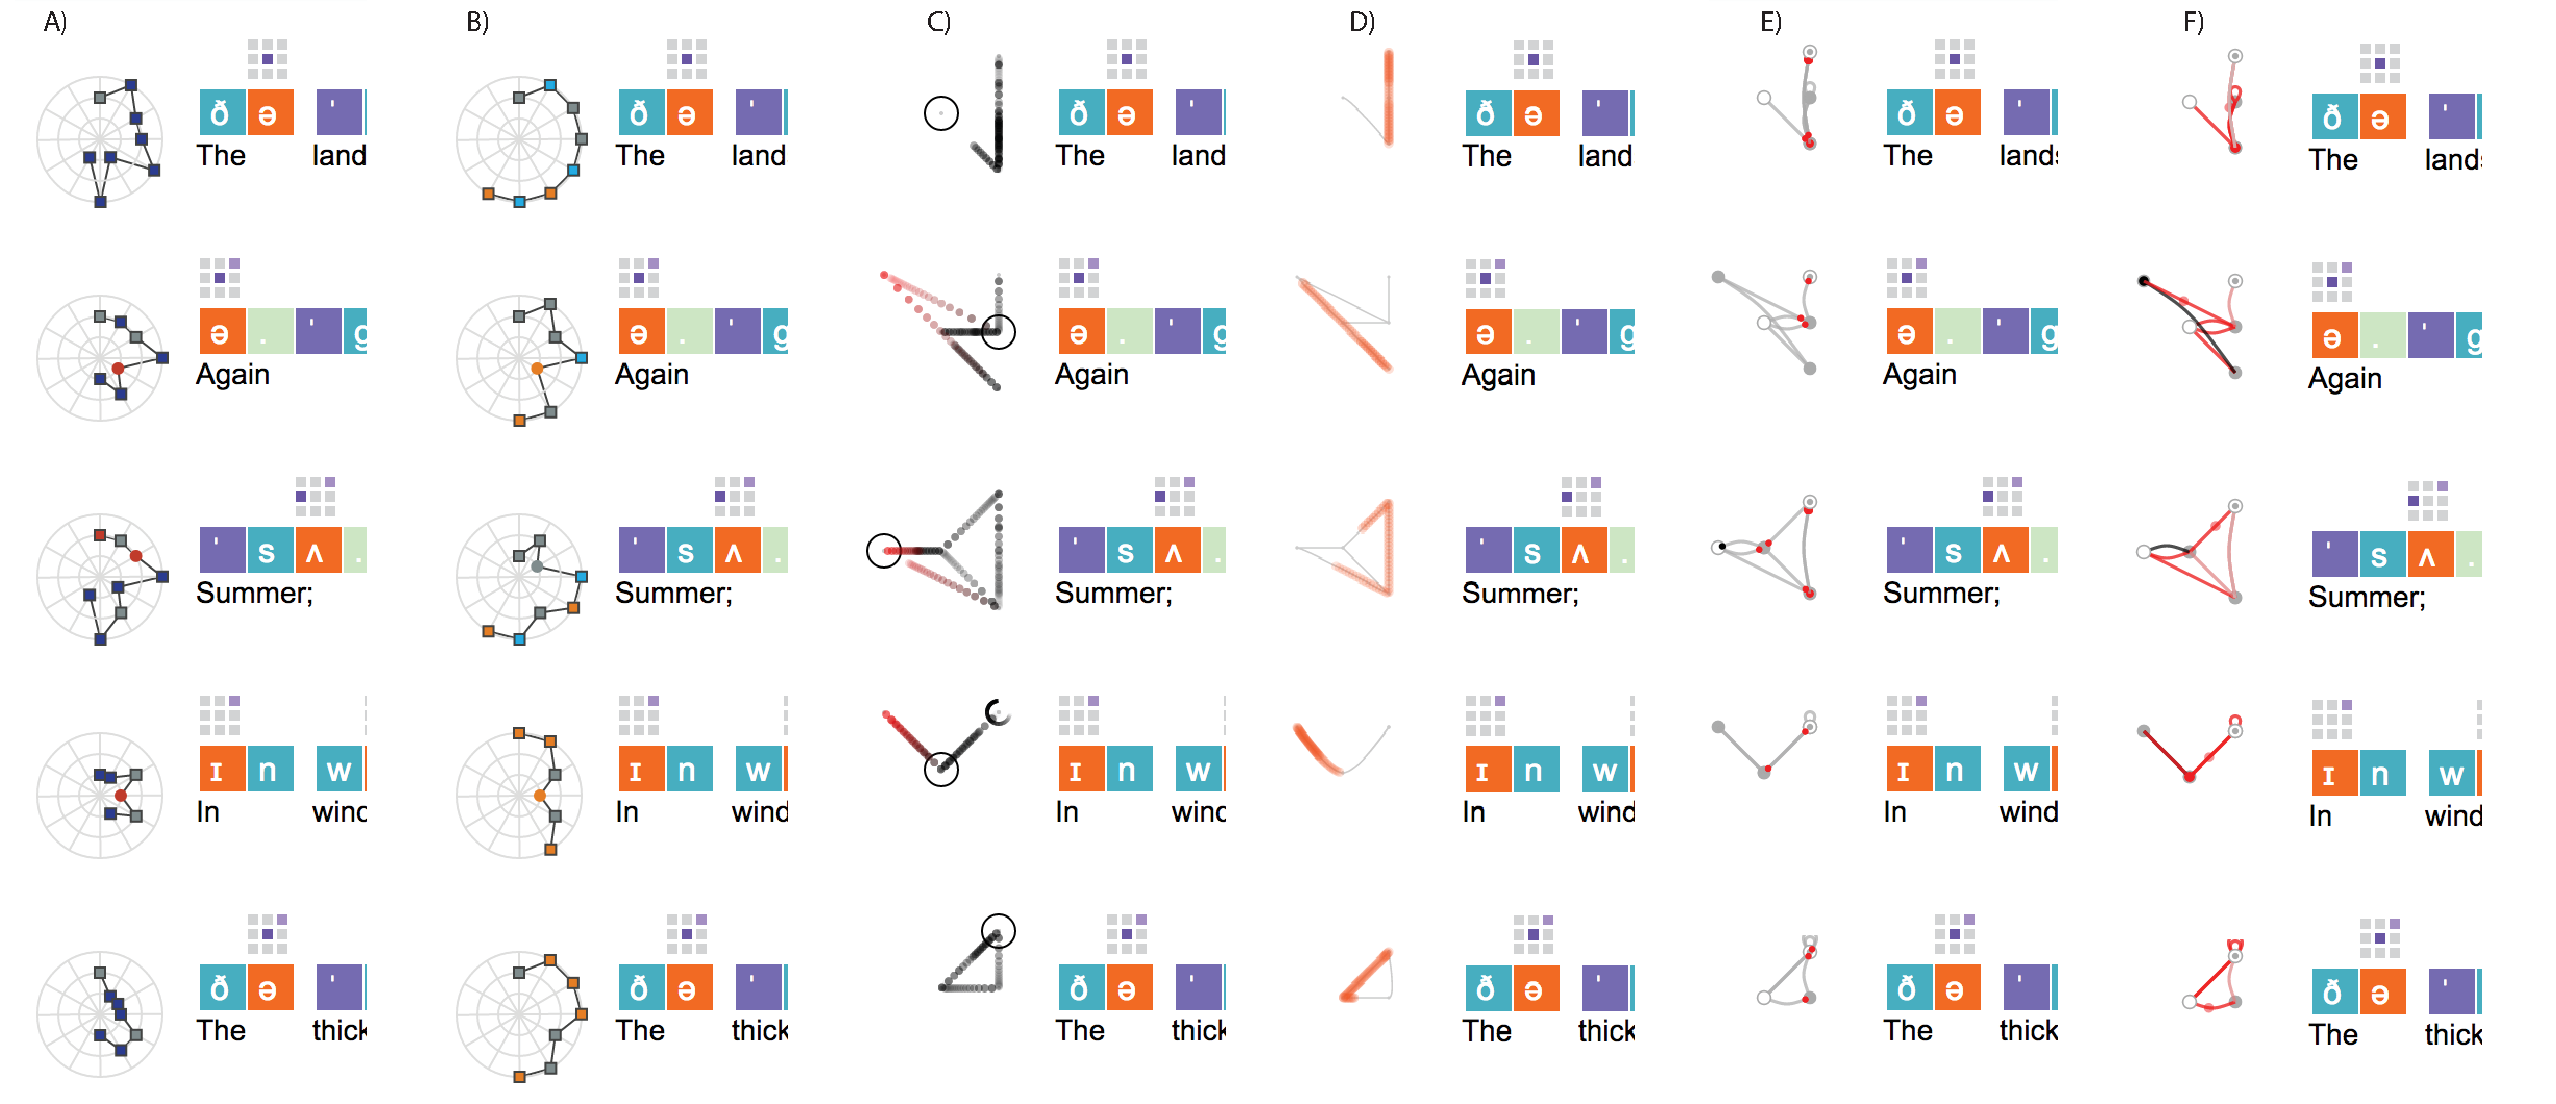
\includegraphics[width=\textwidth]{images/other_glyphs/macros_options}
\caption{Six macro glyphs visualizing five lines of the same poem. 
A) Static radial layout with radial position representing back to front of the mouth.
B) Static radial layout with radial position representing close and open positions of the tongue.
C)-D) Animated transition macro glyphs with trails highlighting previous position. 
E)-F) Animated transition macro glyphs with markers and permanent trails highlighting previous positions.
A video showing the animated glyphs can be found at \url{https://vimeo.com/120620233}.
}
\label{fig:macro_glyph_implementation}
\end{figure}

Figure \ref{fig:macro_glyph_implementation} presents the implementation of the two static macro glyphs, and four variations of the animated macro-glyph, used to visualise five lines of the same poem. 
Due to an understanding that animated glyphs may prove difficult for users wishing to preserve previous transitions, a number of animations were attempted.
Figures \ref{fig:macro_glyph_implementation} C to F represent these different animation strategies to be assessed by expert users.

\subsubsection{Evaluation}

To evaluate the effectiveness of the macro glyph representation, three postgraduate students in English and French literature, and a Professor of Italian literature were invited to an evaluation session. 
The evaluation consisted of a demonstration of the three designs and the variations of the animated glyphs shown in Figure \ref{fig:macro_glyph_implementation}, followed by a questionnaire consisting of forty-three questions, a discussion, and finally an opportunity to change answers based on the discussions and answers they received.

The responses are summarised as follows:
\begin{itemize}
\item \textbf{Static Radial Macro Glyphs}
\vspace{-1mm}
\begin{enumerate}
\item Both types of radial representations are important to scholars depending on the task;
\vspace{-2mm}
\item Helpful in: a) identification of phonetic patterns among lines; and b) differentiation of dynamics and structures in poems;
\vspace{-2mm}
\item Circles and squares work well for differentiating between rounded and unrounded vowels respectively; and
\vspace{-2mm}
\item The logo logical link between the colours used and say open (orange) or closed (cyan) tongue made remembering the colour coding an easier process.
\end{enumerate}
\vspace{-2mm}
\item \textbf{Animated Transitions}
\vspace{-1mm}
\begin{enumerate}
\item Entertaining to watch;
\vspace{-2mm}
\item Intuitive to use when observing the general flow but after some time, the temporal ordering is lost; and
\vspace{-2mm}
\item Opacity as a tool for encoding frequencies is helpful but it can present ambiguity;
\end{enumerate}
\vspace{-2mm}
\item \textbf{Static Transitions with Temporal Highlight}
\vspace{-1mm}
\begin{enumerate}
\vspace{-2mm}
\item Similar to the \emph{Animated Transitions}, it is intuitive, but the ability to track is lost after some observation time;
\vspace{-2mm}
\item Residual line patterns show direction and frequency well, but temporal ordering is not shown; and
\vspace{-2mm}
\item The moving highlight is helpful but not enough to enable the remembering of temporal ordering.
\vspace{-2mm}
\end{enumerate}
\end{itemize}

Although the animated macro glyphs were entertaining for users and did contribute to the analysis of the poem, the most useful macro glyphs for determining the relations between lines of poems were the static representations.
The issues with animation were understood in advance of this work, in particular the problems with depicting temporal information.
However, they still proved useful for depicting overall flow of information. 

\subsection{Poem Viewer}

\begin{figure}[t!]
\centering
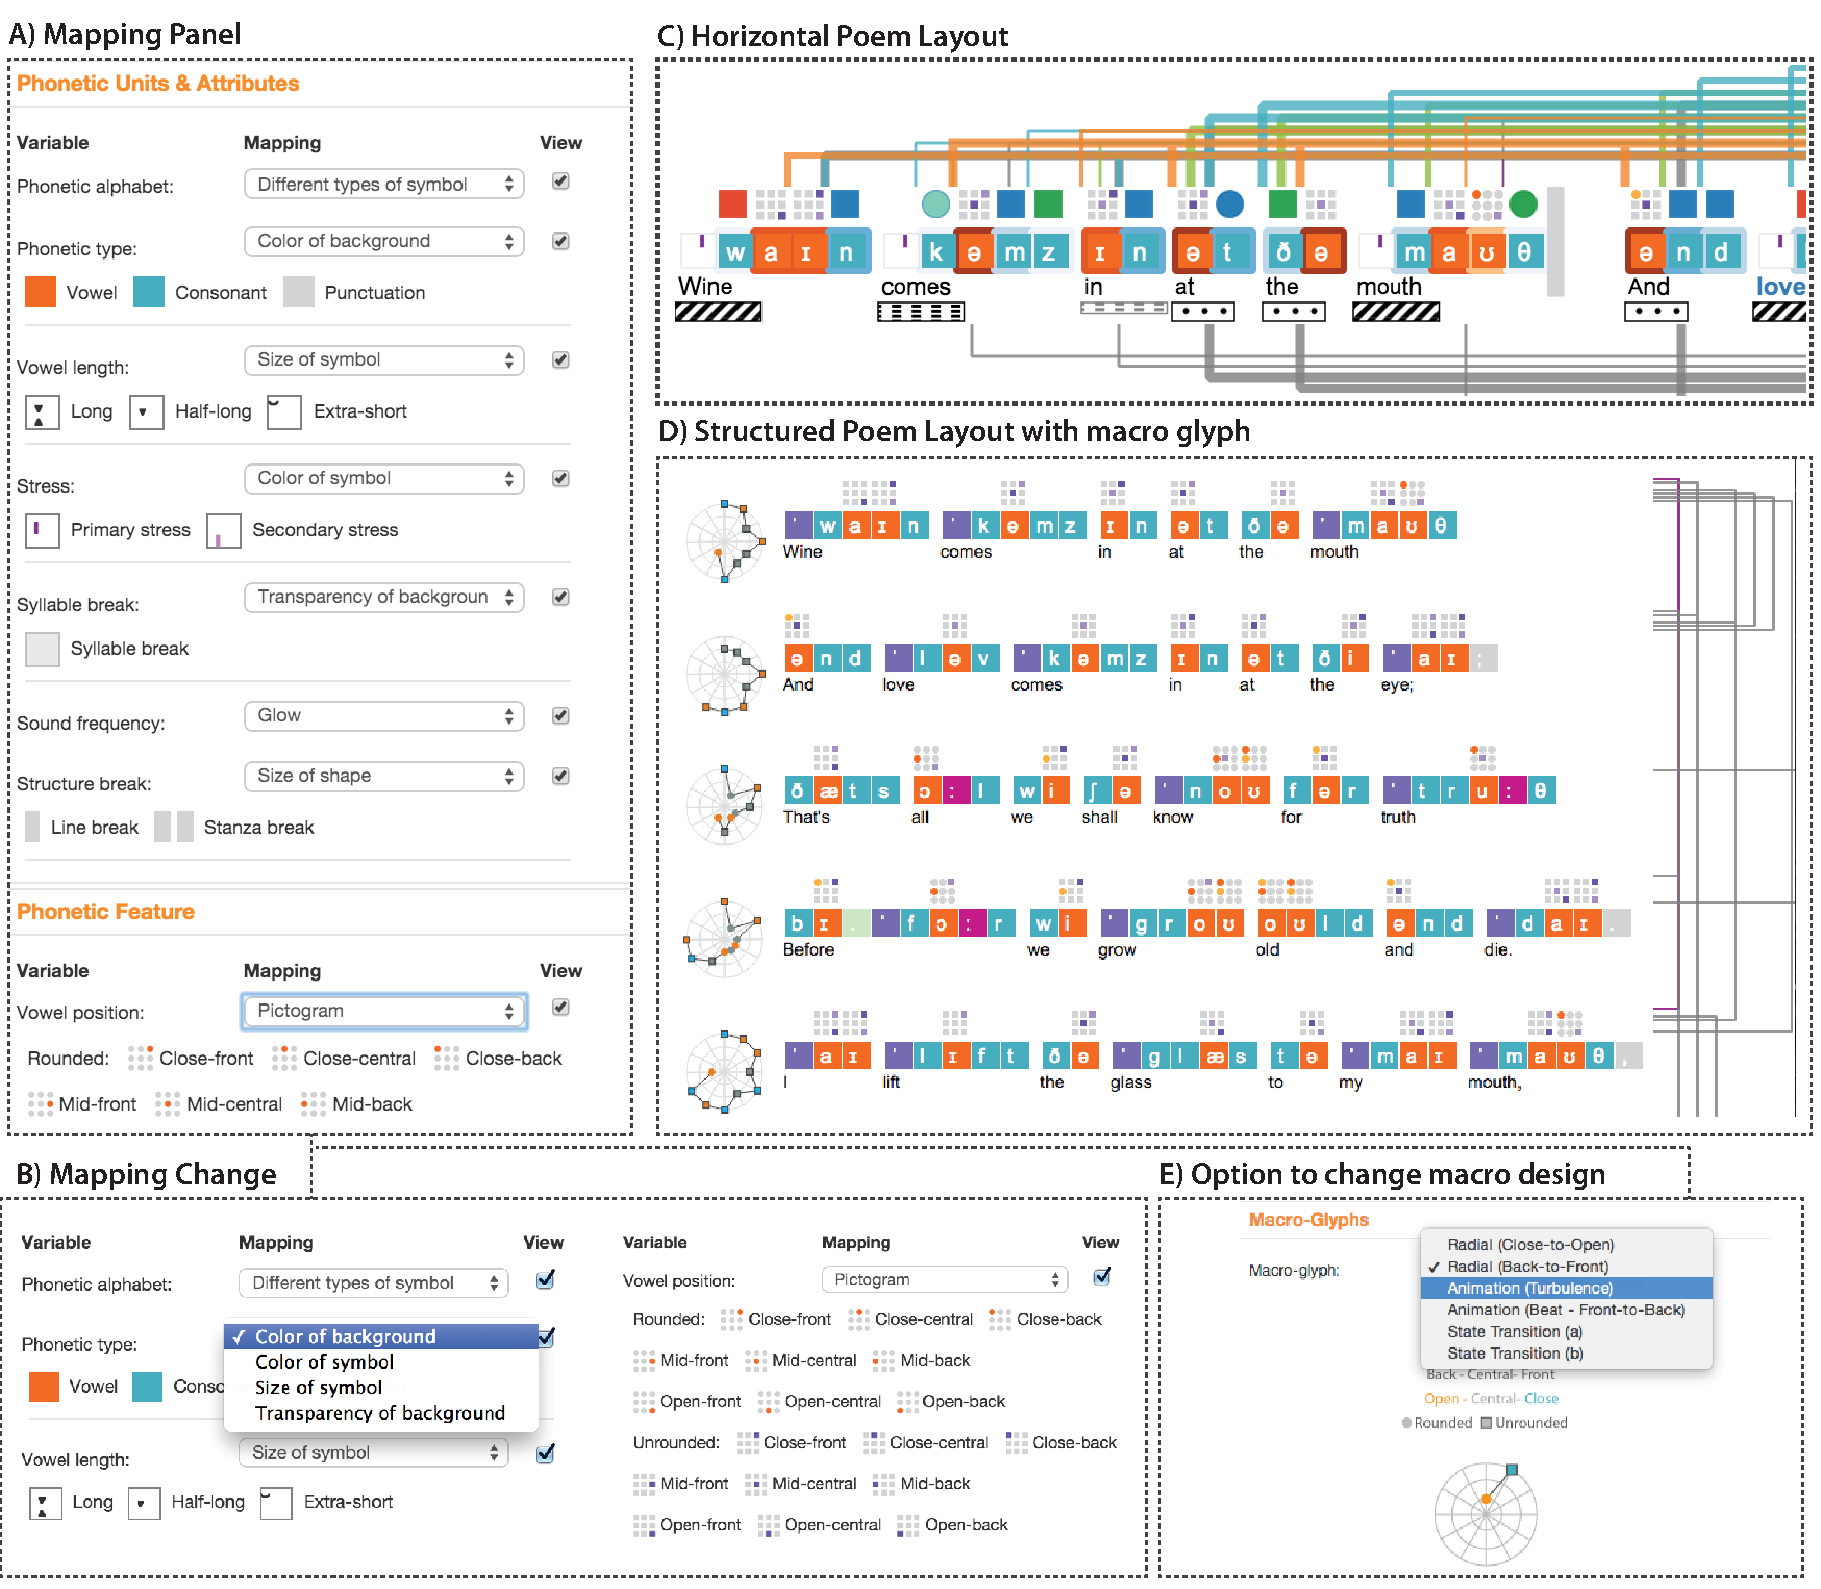
\includegraphics[width=\textwidth]{images/other_glyphs/poemview_overview}
\caption{The Poem Viewer interface.
A) The mapping panel allows users to specify how poem variables are mapped to visual channels.
B) Some examples showing mapping restrictions devised from the rule-based approach.
C) The poem can be viewed horizontally or in its structured layout in D) which also shows the macro glyphs for poem turbulence.
E) A number of macro glyphs, static and animated can be used to visualize the data.}
\label{fig:poem_view_overview}
\end{figure}


Both pieces of work were integrated in PoemViewer \url{http://www.ovii.org/PoemVis/} shown in Figure \ref{fig:poem_view_overview}, an online tool that supports poem upload and visualization functionalities.
Additionally, the interface supports ``rule-based mappings'' so that users can configure visual mappings from poetic variables in a controlled way. 


\newpage
\section{Glyph-based Solutions for File System Visualization}
\label{sec:file_system}
Glyphs are typically small, and are often designed with a high-degree of similarity in order to facilitate mapping consistency, semantic interpretation, learning, and memorisation.
In many applications of spatial or temporal visualization, it is often the case that a large number of small glyphs are displayed on the screen at one time.
For the biological workflows described in Chapters \ref{chap:glyph-tax} and \ref{chap:automacron} for instance, the number of glyphs on the screen can be in the thousands.
In this chapter we are focused on the \emph{differentiability} of such glyphs and solutions to potential perceptual errors in their observation and exploration.

Figure~\ref{fig:reduction_degradation} presents some example cases that may render some glyphs indistinguishable. 
For example, zooming out in data exploration can reduce glyph size significantly.
This could make some shapes (\eg, circle and hexagon) and textures appear similar, while confusing the categorisation of sizes (\eg, big, medium, small).
Additionally, environmental lighting conditions, and printing or photocopying facilities can cause colour and greyscale degeneration.
Such changes would make some glyphs indistinguishable, and also confuse associations between different colours or shades of grey and the concepts they represent.
A dynamic legend may help alleviate the confusion about various mappings, however these legends demand regular attention from users.
This extra lookup action incurs additional cognitive load due to the effort required for visual search and memorisation of unstable mapping keys.
These issues may be compounded by colour- or change-blindness, short- or long-sightedness, clustering, occlusion, and distortion.

\begin{figure*}[t]
\begin{center}
%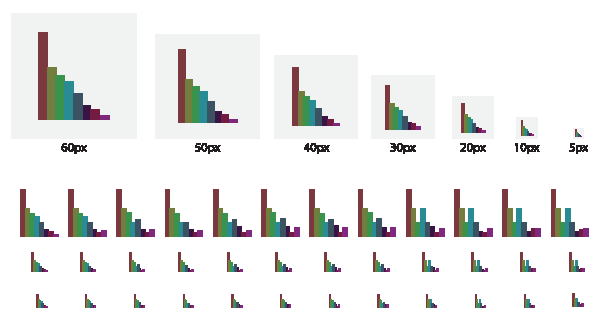
\includegraphics[width=0.9\textwidth, height = 3in]{problems}
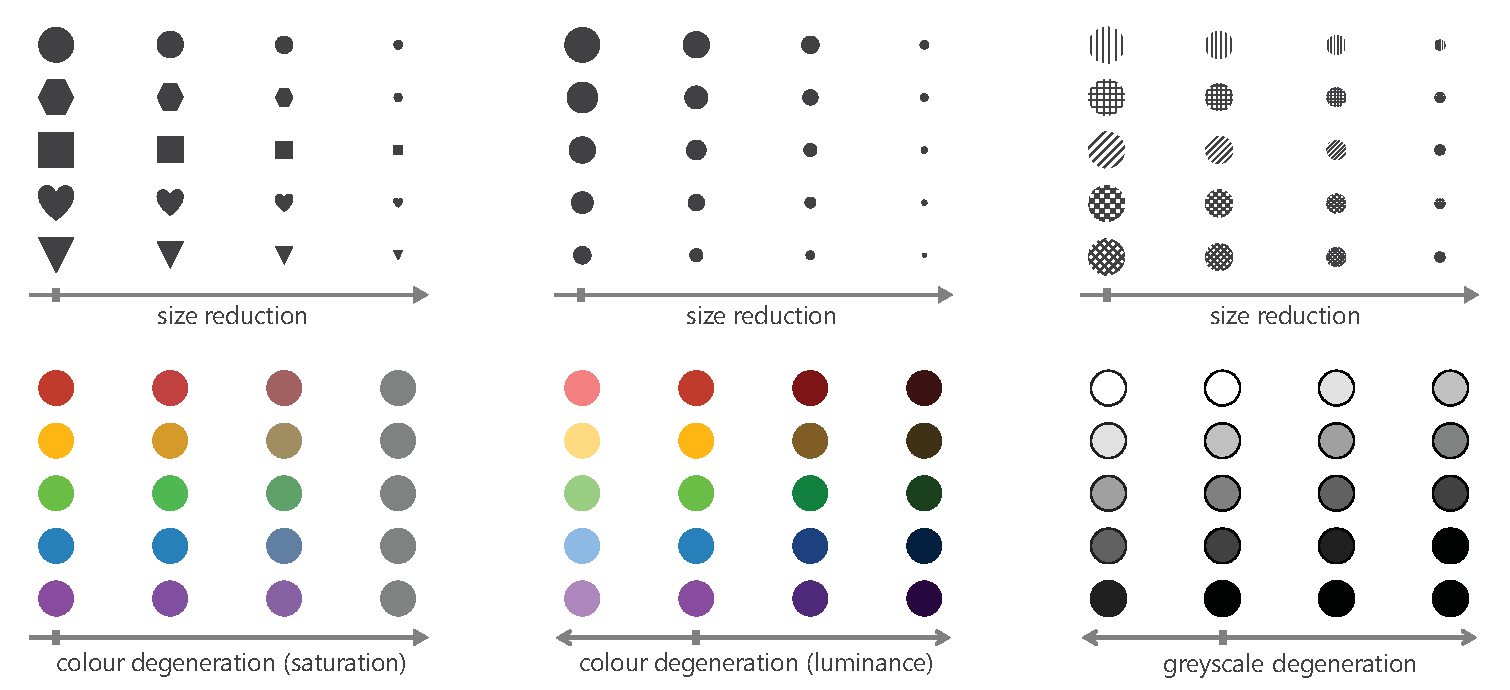
\includegraphics[width=0.95\textwidth]{images/filesystem/Unsafe}
\end{center}
\caption{Three different types of quality degeneration applied to several glyphs, each of which is encoded using a single retinal variable.
The original quality is indicated by a marker on the $x$-axis.
All variations of degeneration result in perception difficulties, however the effect is more so with size, saturation and luminance adjustments.}
\label{fig:reduction_degradation}
\end{figure*} 


\subsection{Background}
Perceptual guidelines discussed throughout this thesis can be adopted for more effective visualization. 
By using the correct data type to retinal variable mappings, prioritising dimensions based on their importance to tasks, and ensuring separability of dimensions, the glyph design process can be improved.

%This chapter extends on those foundations to provide a computation
Glyph designers will often use their creative intuition to ensure the diversity and legibility of different glyphs as is seen within the icon and font design communities.
Much of the work presented in this thesis so far has focused on the use of computation in combination with design principles to systematise the glyph design process in terms of what visual channels should be used and where. 
A further research question however would be \emph{``Is there a systematic approach to design a fail-safe glyph set?''}.

This work proposes a conceptual framework to optimise the design of a set of glyphs to provide a systematic way of ensuring fail-safe glyph encoding.
The framework is based on the \emph{Hamming} distance (Section \ref{sec:hamming}).
Due to the subjective nature of many design aspects, we introduce the concept of the \emph{quasi-Hamming distance} (QHD) (Section \ref{sec:qhd}).
Using this idea, we are able to transition from a qualitative assessment of perceptual distances in a design to a more quantifiable assessment based on this new metric.
For instance, when the minimal Hamming distance for a glyph set is one, the glyph set is vulnerable to ``noise'' during observation and exploration. 
If the minimal Hamming distance is two, the glyph set facilitates some error detection, whereby the viewer can use interaction (\eg, zooming-in, or looking at the legend) to investigate the error.
When the minimal Hamming distance is three or more, the glyph set facilitates some error correction at the receiving end.
This enables us to adjust the design to ensure a minimal Hamming distance among each glyph in a set of glyphs.
In addition to this novel concept for glyph design, this work makes the following additional contributions:  
%
\begin{itemize}
\vspace{-2mm}
\item
We outline several methods for estimating the QHD, and present two proof-of-concept of experiments for estimating the QHD based on manual grading by human participants, and through use of image-comparison metrics (Section \ref{sec:qhd}).
\vspace{-2mm}
\item
We present a case study on visualising file system events, where glyphs were designed to facilitate error detection and correction, and were evaluated by human participants and image-comparison metrics (Section \ref{sec:casestudy}).
\vspace{-2mm}
\item
We demonstrate the fail-safe file system event glyphs in a new visualization environment using event log data captured from Dropbox, a real-world distributed file sharing system \footnote{\url{www.dropbox.com}}.
\end{itemize}

\subsubsection{Hamming Distance}
\label{sec:hamming}

In information theory and data communication, a \emph{code} consists of a finite set of \emph{codewords}, each of which is a digital representation of a letter in an alphabet.
In the context of binary encoding, the \emph{Hamming distance}, proposed by Richard Hamming in 1950 \cite{Hamming:1950:Bell}, is a measure of the number of bit positions in which two codewords differ.
Considering all pairs of codewords in a code, the minimal distance is referred to as the minimal Hamming distance of the code.
In communication, there are two main strategies for dealing with errors that occur during transmission.
\emph{Automated error detection} allows the receiver to discover that any error has occurred and to request a retransmission accordingly.
\emph{Automated error correction} enables the receiver to detect an error and deduce what the intended transmission must have been.
Hamming defined the following principle:

\begin{figure}[h!]
\begin{center}
\includegraphics[width=\textwidth]{images/filesystem/latest/Hamming1}
\end{center}
\caption{Principles of error correcting codes.
A) A code with no error detection where every code is valid. No way of detecting errors and no way of correcting them.
B) A code with a distance of two bits between valid codes can detect errors but cannot correct since one change in any position will result in a valid code (knowing what changed is difficult).
C) A code with a distance of three bits between valid codes can detect errors and correct them.}
\label{fig:hamming}
\end{figure}

\noindent \textbf{Theorem.} A code of $d+1$ minimal Hamming distance can be used to detect $d$ bits of errors during transmission. A code of $2d+1$ minimal Hamming distance can be used to correct $d$ bits of errors during transmission~\cite{Hamming:1950:Bell}.

For example, given a three-bit code as illustrated in Figure~\ref{fig:hamming}, there are eight possible codewords.
One may select a subset of these codewords to construct a code with its minimal Hamming distance equal to two bits or three bits.
Figure~\ref{fig:hamming} B) shows such a code with four valid codewords and a minimal Hamming distance of two bits.
This code can detect one-bit errors since any change of a valid codeword by one bit would result in an invalid codeword, which would lead the receiver to discover the error.
Figure~\ref{fig:hamming} C) shows another code, with two valid codewords and a minimal Hamming distance of three bits.
This code can detect two-bit errors and correct one-bit errors.
When a valid codeword (\eg, 111) is changed by one bit during transmission (\eg, 110), the receiver can detect such an error and recover the intended codeword based on the nearest neighbour principle.
Of course, if a two-bit error occurred during transmission, the receiver would be able to detect the error but could not make a correct ``correction''.
Nevertheless, if it is known that two-bit errors are likely to occur then this should either be used as only an error detection code, or a code with a larger minimal Hamming distance should be used instead.

\subsubsection{A Quasi-Hamming Distance for Glyph Design}
\label{sec:qhd}

One can consider a set of glyphs as a code, and each glyph in the set is a valid codeword.
On presenting a glyph-based visualization to a user, there may be errors in the display and perception of a glyph.
If a viewer can detect that a perceived glyph is not quite ``right'', conscious or unconscious effort can be made to correct such an error.
Conscious effort, an analogy of error detection and repeated transmission, may typically include zooming in to have a close look, or consulting the legend.
Unconscious effort, an analogy of error correction, may include some Gestalt effects \cite{Chen:2014:CGF}, and inference from other visual information \cite{Rheingans:1995:PIV}.
Figure~\ref{fig:glyph_hamming} shows two example glyph sets, each with eight codewords.
Given the two display errors shown on the left, where an arrow glyph is skewed in a distorted printout, and a shape glyph is occluded by another shape.
Both errors can be detected, although the error for the arrow glyph will require more conscious effort to correct, although in this case that would be impossible due to the small distance between each glyph in the set. 
The star glyph can be corrected unconsciously due to Gestalt effects in combination with the greater distance between each of the glyphs.
These examples would suggest that it is possible to establish a conceptual framework, similar to the Hamming distance for error detection and error correction in glyph-based visualization.

\begin{figure}[t!]
\begin{center}
\includegraphics[width=\textwidth]{images/filesystem/latest/QHD}
\end{center}
\caption{Two examples that illustrate the phenomena of error detection and error correction in glyph-based visualization. (Above) A viewer may sense that the glyph on the left may not be correct in a distorted visualization, and consult the legend to correct the error. (Below) A viewer may unconsciously perceive the glyph on the left as a star shape due to Gestalt effects and apriori knowledge about the glyph set.}
\label{fig:glyph_hamming}
\end{figure}


Understandably, measuring the distances and errors in visual perception is not as simple as measuring those represented by binary codewords.
We propose an approximated conceptual framework based on the principle of Hamming distance, which we call a \emph{Quasi-Hamming Distance} (QHD).
The term ``quasi'' is used to show that the distance measure is an approximate, and that the quantitative measure of perceptual error is also approximated.
Therefore, the main research questions are:
i) can we establish a measurement unit common to both measures?; and
ii) given a glyph set, how can we measure the distance between those glyphs?\\

\noindent\textbf{Can we establish a measurement unit common to both measures?} A ``bit'' can be used as the common unit for both distance and error measurement.
Consider an ordered retinal variable, such as brightness or length, as a code $C$.
Theoretically, $C$ can have a set of codewords $\{ c_1, c_2, \ldots c_n \}$ such that the difference between two consecutive codewords is the just-noticeable difference (JND) of this retinal variable.
We can define the QHD between each pair of codewords $c_i$ and $c_j$ as $|i-j|$ bits.
During display and visualization, if $c_i$ is mistaken for $c_j$, we can call this a $d$-bit error where $d=|i-j|$.
Now let us extend this concept to a less ordered retinal variable (\eg, colour hue).
Theoretically, we can construct a code $C$ by uniformly sampling the space of the retinal variable (\eg, the CIE L*a*b* colour space) while ensuring that every pair of samples differ by at least the JND of this channel.
These codewords can be organised into a network, where the distance between any two codewords can be approximated proportionally according to the JND (\emph{i.e.}, JND = 1 bit).
The possible perception error rate with a code that maximises the number of codewords based on JND is likely to be very high.
In practice, a glyph set is designed using a small subset of visual channels.
However, it is more common to use several visual channels in the multivariate.
Therefore a QHD measure based on JND would be too fine to use in practice, although JND can provide an \emph{absolute reference measure} once measures for the visual channels used in visualizations have been obtained.\\

\noindent\textbf{Given a glyph set, how can we measure the distance between glyphs?} One may consider using the following methods:
\begin{enumerate}
\vspace{-1mm}
\item \textbf{Estimation by expert designers.} This practice has existed in design exercises such as the development of traffic signage (discussed in Chapter \ref{chap:related_work}, Section \ref{sec:relwork_glyphs}) and icons in user interfaces.
To formalise this practice, designers can explicitly estimate and label the distance between each pair of glyphs in a glyph set.
While this approach may be most convenient to the designers, its effectiveness depends very much on the experience of the designers concerned and it is easy to overlook certain types of display and perception errors;
\vspace{-1mm}
\item \textbf{Crush tests.} This test was introduced in Chapter \ref{chap:glyph-tax} to simulate how changes in size affect the perception of glyph features.
By simulating the various causes of perception error, such as those illustrated in Figure~\ref{fig:reduction_degradation}, we can determine the level at which glyphs become indistinguishable.
The corresponding level of degeneration can be defined as a QHD.
While this approach would yield more consistent estimation of a QHD, more research would be required to compile a list of different causes of errors and define coherent levels of degeneration across different causal relationships;
\vspace{-1mm}
\item \textbf{Task-based evaluation.} Similar to (2), one can simulate different visualization conditions, enlist users to perform their tasks, measure their performance, and transform performance measures to a QHD.
On one hand, this approach is perhaps most semantically meaningful for a particular glyph set in a specific application context.
On the other hand, the performance measures collected may feature many confounding effects, while there may only be a small number of users available for such an evaluation;
\vspace{-1mm}
\item \textbf{User-centric estimation.} One may conduct a survey among human participants about how easy or difficult it is to differentiate different glyphs. By removing task-dependency in (3), more participants can be involved in such a survey, yielding a more reliable estimation of the QHD.
Recent efforts have taken place to crowd source distances between simple shapes, colours, and sizes to create what are called \emph{Perceptual Kernels} \cite{demiralplearning}; and
\vspace{-2mm}
\item \textbf{Computer-based similarity measures.} A large collection of image similarity measures exist in the literature~\cite{Sahasrabudhe99, Eler08}.
%It is likely that we will be able to find measures that are statistically close to a user-centric estimation in the long term.
However, there are few metrics available that are designed for measuring the glyph similarity.
A good long term approach would be finding metrics that are statistically close to a user-centric estimation.
\end{enumerate}

To demonstrate the feasibility of estimating a QHD, we conducted two proof-of-concept experiments based on methods (4) and (5).
We conducted a survey among twenty participants, all of whom are either employees or students at University of Oxford.
About 50\% encountered glyph-based visualization in their course or work.
After a brief introduction, the participants were asked to rate how difficult or easy it was to differentiate 104 pairs of glyphs using an integer scale from 0 to 10.
The survey was conducted during an informal lunch, where pizzas were served.
No cash payment was involved.
The results of one participant were considered an outlier and were not included in the statistics.

\begin{figure*}[t!]
\begin{center}
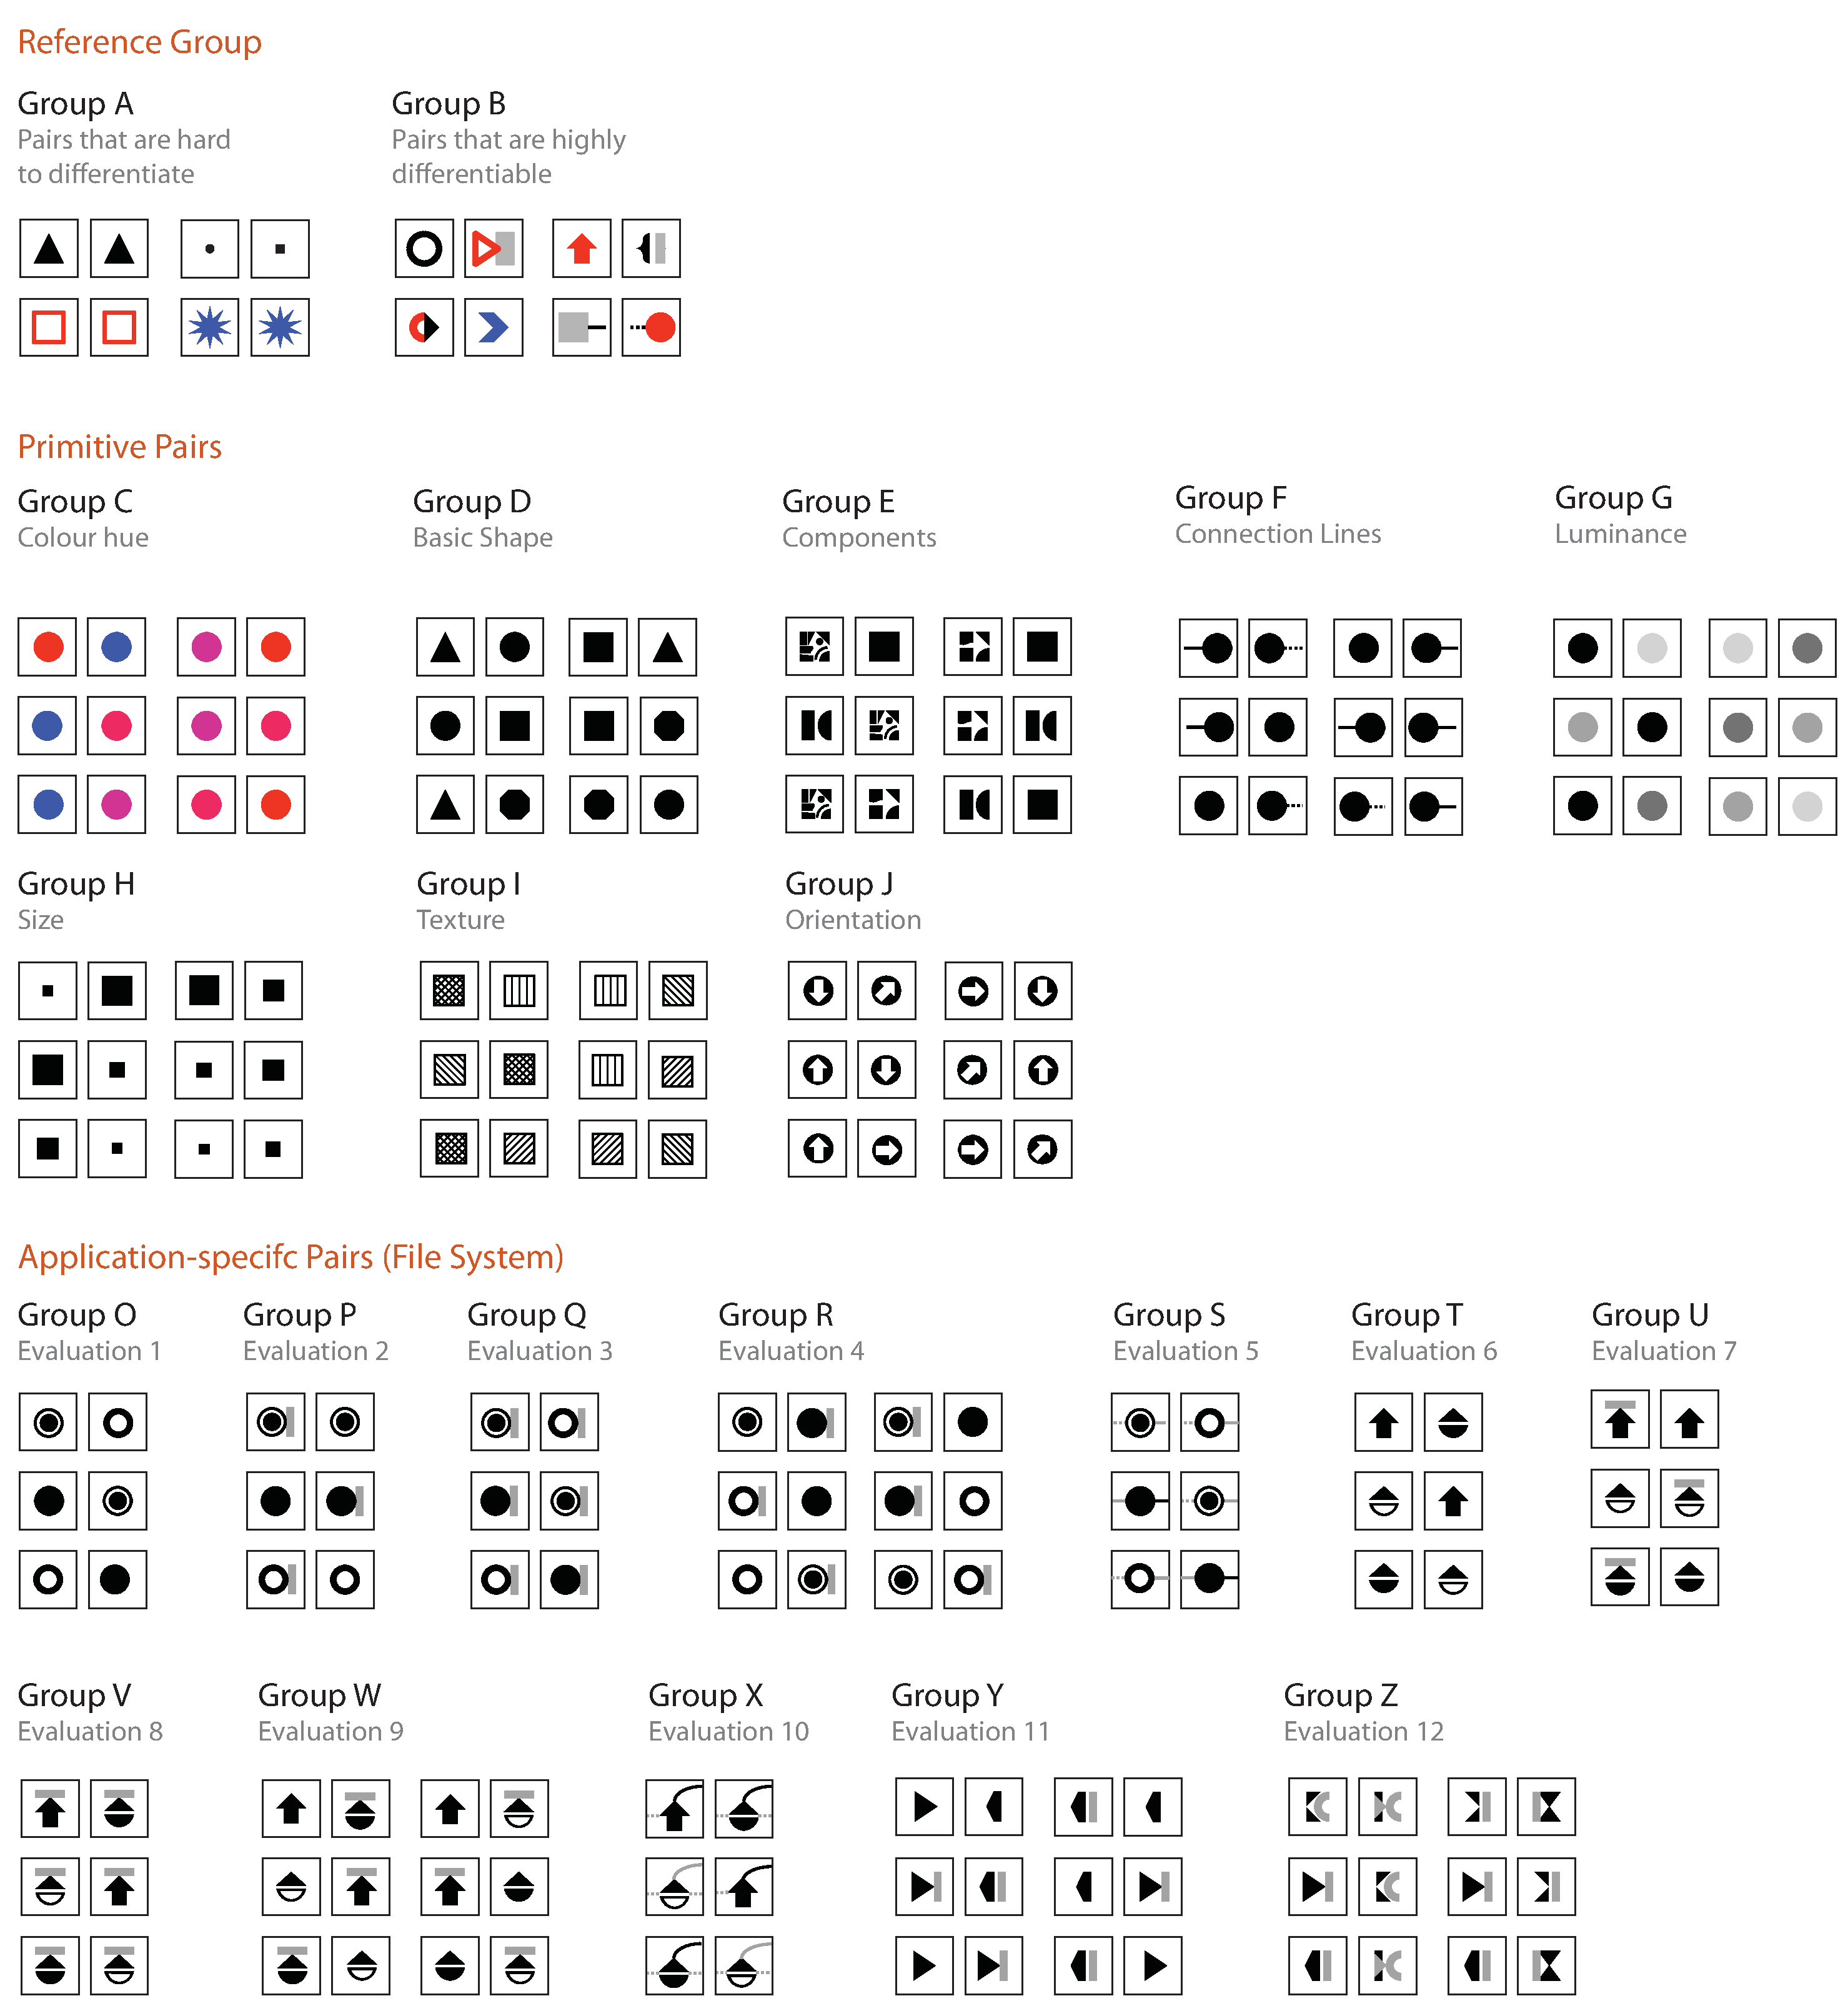
\includegraphics[width=\textwidth]{images/filesystem/evaluation_groups}
\end{center}
\caption{104 stimulation pairs are split in to three groups representing: the reference group; primitive pairs; and application-specific pairs.}
\label{fig:evaluation_groups}
\end{figure*}


Illustrated in Figure \ref{fig:evaluation_groups} are the 104 stimuli pairs divided into three categories: eight \emph{reference pairs}; forty-eight \emph{primitive pairs}; and forty-eight \emph{application-specific pairs}.
We will discuss the last category in detail in Section \ref{sec:application}.
The ninety-six primitive and application-specific pairs were mixed together in a randomised order.
The eight reference pairs were placed at positions 1, 2, 35, 36, 69, 70, 103, and 104 to help participants regularise their scores and to enable a temporal consistency check.

The reference pairs are divided into two groups.
Group A consists of four pairs of very similar glyphs, and Group B consists of four pairs of very different glyphs. 
We expected that participants would assign very low scores (difficult to differentiate) to those in A and high scores (easy to differentiate) to those in B respectively.
We placed one pair from A and one from B at regular intervals.
The average scores for the four pairs in group A are (0.0, 0.4, 1.4 and 2.8) respectively and those for group B are (9.3, 9.0, 8.9, 9.7) respectively, indicating that statistically, they have served as references for the minimal and maximum QHD in this survey.

The primitive pairs consist of eight groups for estimating the QHD in relation to eight visual channels, namely colour hue, shape, components, connection lines, luminance, size, texture, and orientation.
Each group has six pairs of stimuli, facilitating pairwise comparison of four different codewords for each channel.
For hue and luminance channels, after choosing the first and fourth codewords, we used a perceptually uniform colour model (Hunter's Lab) \cite{hunter1958photoelectric} to determine the second and third codewords at 50\% and 75\% distance from the first.
The upper part of Figure~\ref{fig:eval_glyph_scores} E shows a small selection of survey results, where we converted the $[0, 10]$ score range to a $[0, 5]$ QHD range.
We considered any QHD $<2$ as potentially risky for error detection, and any QHD $<3$ as potentially risky for error correction.

\begin{figure*}[t!]
\begin{center}
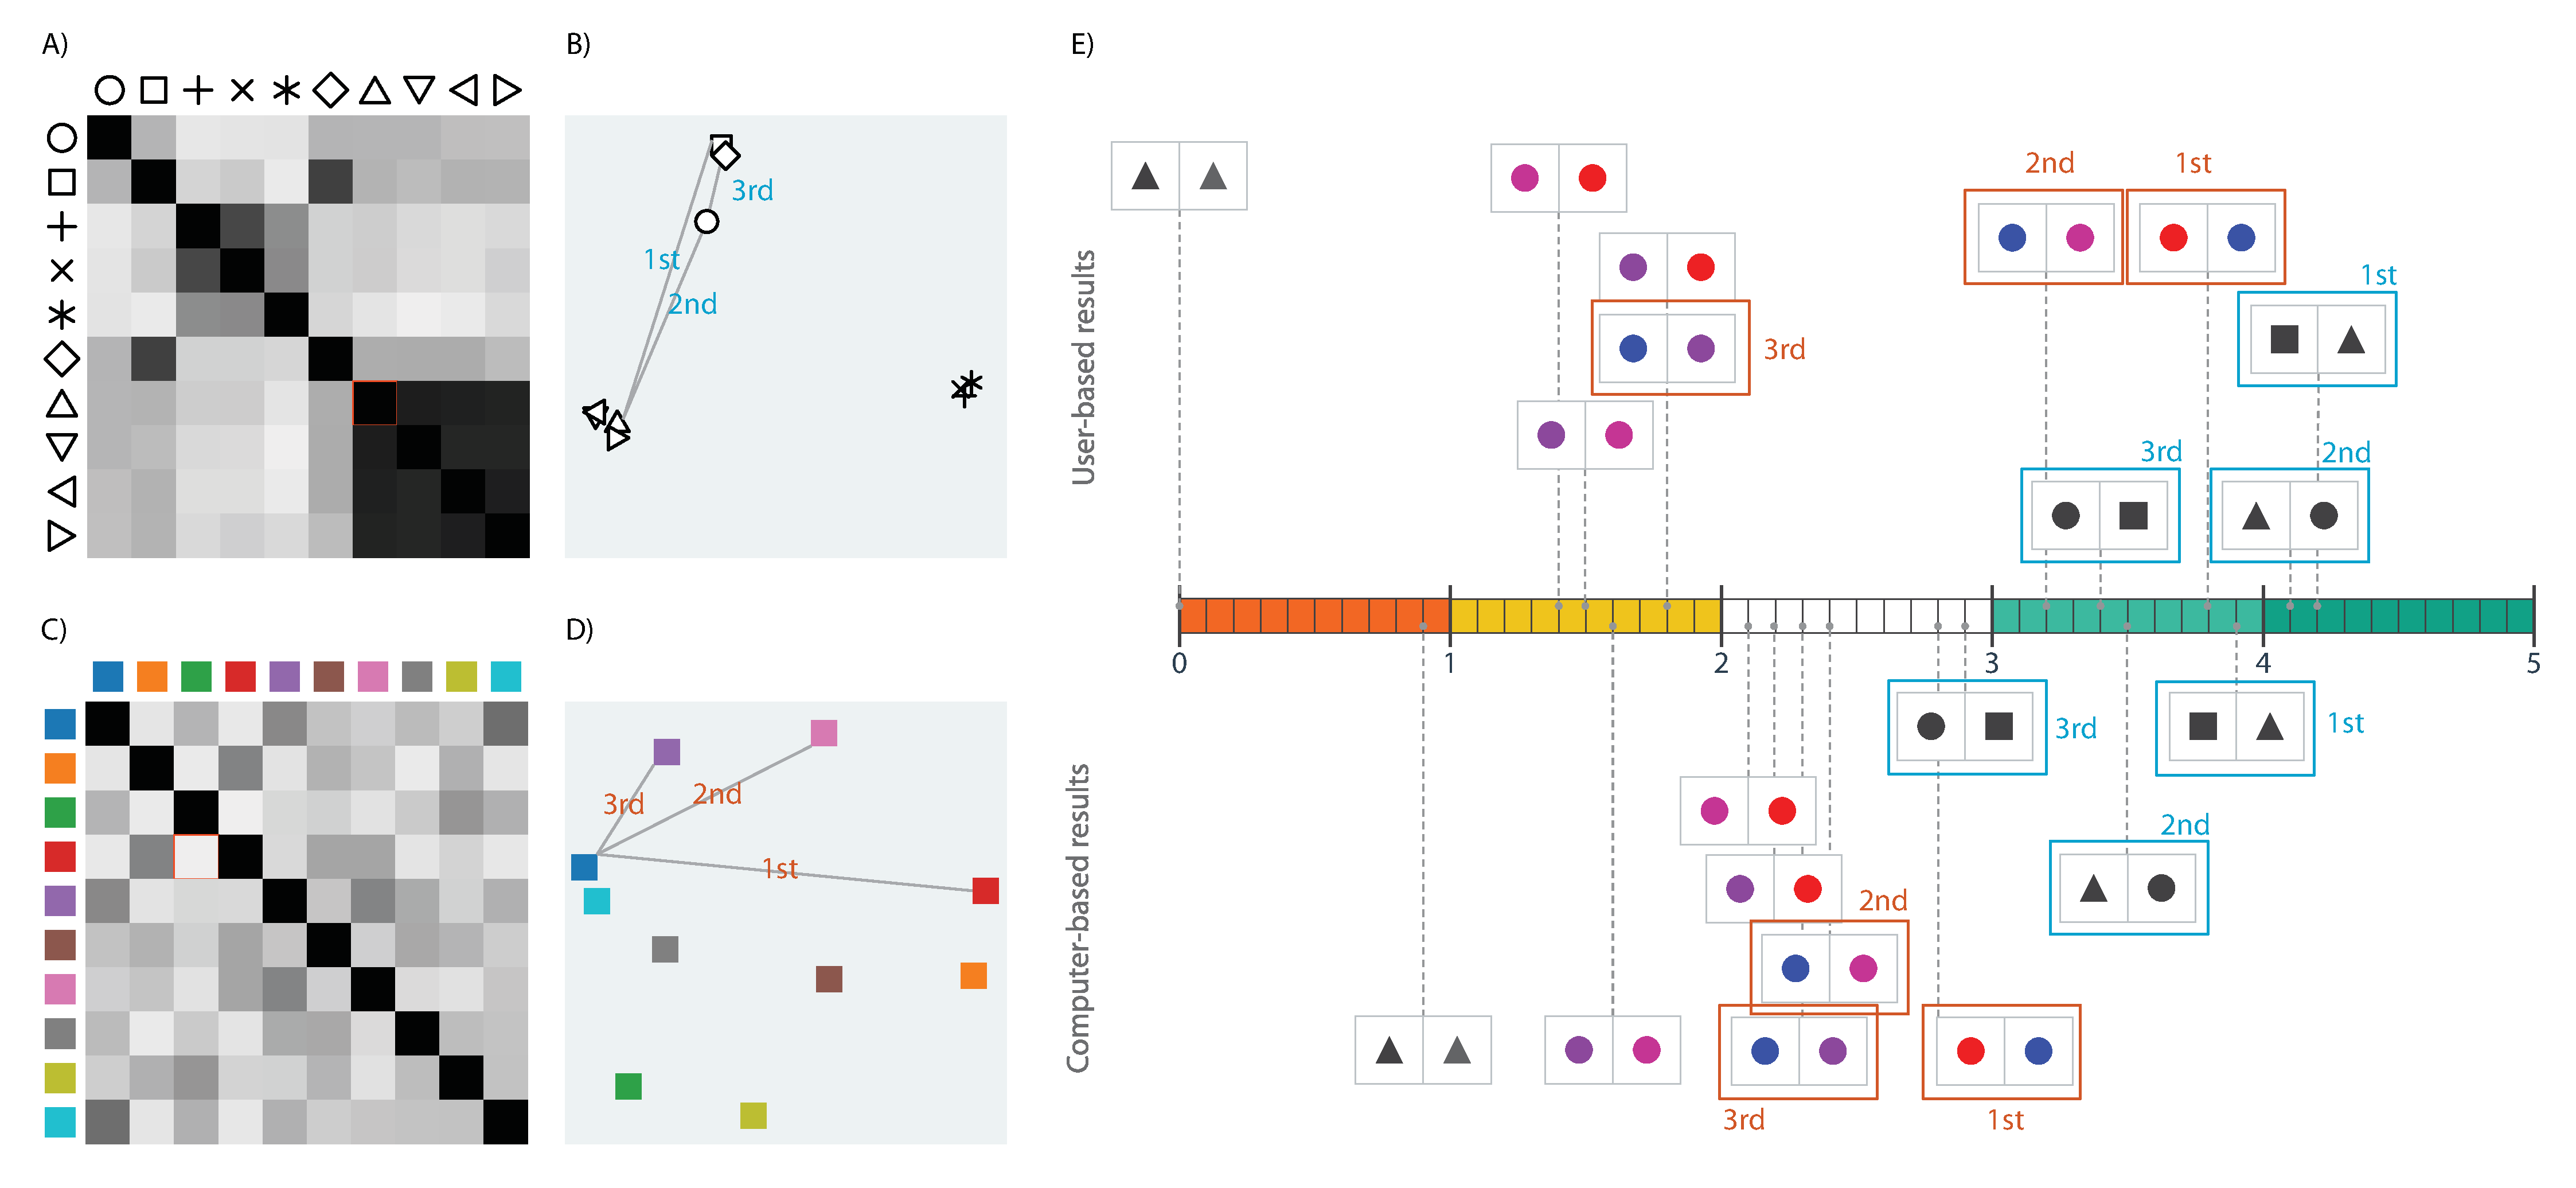
\includegraphics[width=\textwidth]{images/filesystem/perceptual_kernal_validation}
\end{center}
\caption{Reproduced figures from work by Demiralp \etal \cite{demiralplearning} (A-D) with respect to results from analyses in this work (E).
A) Distances between colours shown as a heat map.
The higher the similarity, the darker the square.
B) Shapes arranged in 2D space by their similarity. This is calculated using multidimensional scaling (MDS) of the perceptual kernel.
C) Distances between colours shown as a heat map.
D) Colours arranged in 2D by their similarity (again created from MDS of their perceptual kernel).
E) Results from our user-based and computation-based analyses.
The results are correlated with results from \cite{demiralplearning}.
The top three perceptually distant shapes and colours are marked across the results.}
\label{fig:eval_glyph_scores}
\end{figure*}

In our second experiment, we measured the similarity between each pair of glyphs using a computer-based metric.
This metric combines differences in pixel colour with spatial occupancy.
The former captures a variety of feature differences such as colour, luminance, size, and orientation.
The difference is defined as the mean Euclidean distance between all corresponding pixels in the two images representing the pair of glyphs.
The latter captures some location-invariant features such as spatial occupancy, and is defined as the difference between the numbers of pixels with $\leq 80\%$ luminance.

Both difference measures are first normalised to the $[0, 1]$ range, and are then scaled to the QHD range from the user-centric survey, before being combined into a single metric.
The lower part of Figure~\ref{fig:eval_glyph_scores} E shows the computed similarity measures for the same selection of stimuli pairs.

\subsection{File System Event Visualization}
\label{sec:casestudy}

The problem of visualizing file systems plays a significant role in the short history of computer-assisted visualization.
In 1991, Johnson and Shneiderman, who were motived by the need to visualise the structure of a file system, published their seminal paper on treemaps~\cite{johnson91}.
Today, not only are file systems larger, they are also shared by many more users.
One important aspect of a file system is to support collaborative activities, such as sharing files within multi-partner projects, or developing software with a team geographically distributed programmers.
While there are text-based mechanisms for recording events in relation to a file system or a specific folder, the amount of data contained in typical log files can easily escalate to the point where it becomes too overwhelming for anyone to read.
To our knowledge, there is no effective visualization technique for allowing users of such collaborative environments to observe events in a cost-effective manner.

In this case study, we designed and developed a novel glyph-based visualization tool for observing events in a file system.
There are several technical challenges.
Firstly, the hierarchical nature of the file system needs to be depicted so that the spatial context of where a particular event has occurred can be identified.
Secondly, the temporal information about events needs to be conveyed so that the activity ordering can also be observed and reasoned.
Thirdly, there are a wide range of activities (\eg, copying a file, modifying a file) that are typically performed, which would need to be distinguishable in a visualization.
Finally, the visualization should be able to support collaborative environments by depicting activities by a number of users.

\begin{figure*}[t!]
\begin{center}
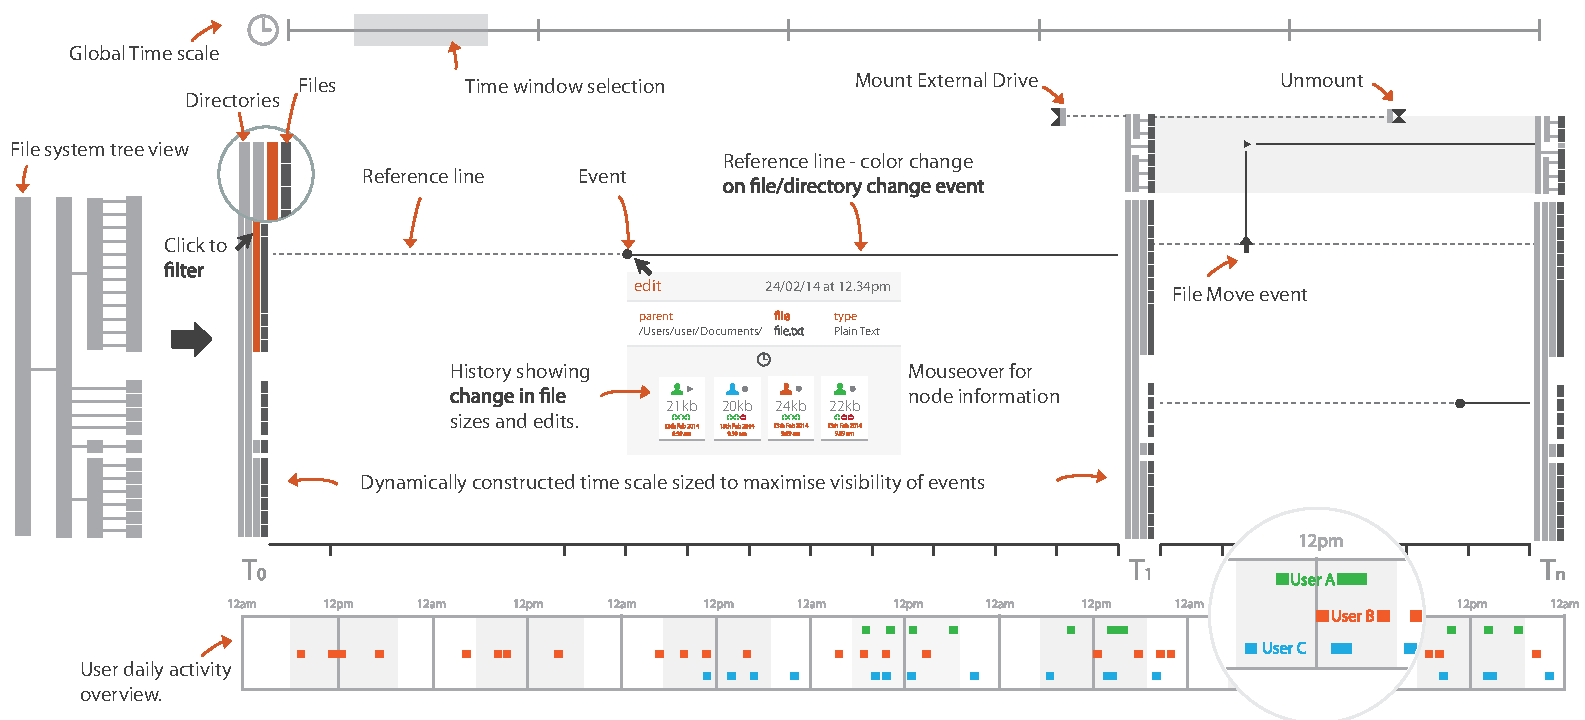
\includegraphics[width=\textwidth]{images/filesystem/system_overview}
\end{center}
\caption{We use a timeline approach with a condensed file system hierarchy at the left of the visualization.
File system activities are depicted by glyphs on the timeline, with connecting lines to show their place in the file system.
Keyframes are displayed to depict significant changes to the file system hierarchy, or at user-specified time intervals.
Interaction with the mouse displays a context aware box, with detailed information on the selected file, directory, and activity.}
\label{fig:system}
\end{figure*}

Figure~\ref{fig:system} presents an overview of the adopted visualization design.
The visualization consists of a number of different components:
\begin{enumerate}
\item \textbf{Central Panel}. The main activity window where events performed on the file system are displayed on a timeline using glyphs. 
To the far left is the file system tree view, which represents the file system using a traditional tree representation where directories are shown as light grey nodes and files shown as dark grey nodes.
Since most directories are likely to contain files, leaf nodes are typically file objects.
This tree is shown as a condensed display to the left of the main timeline and serves as a reference to the spatial context of the file location.
File system events are positioned corresponding to the file system hierarchy.
Connected lines are displayed relating file activities back to a position in the file system hierarchy.
For events that involve a change in the file system hierarchy, such as copying or moving files, these connecting lines also indicate the new position of the file.
The condensed file hierarchy also serves as a ``keyframe'', where the current state of the file system hierarchy is shown, either after a significant change to the hierarchy (\eg, copying files, or mounting an external drive), or at a particular time interval specified by the user.
Finally, the file hierarchy can also be used to select the directory of interest that should be shown on the visualization.
This provides a mechanism for ``zooming in'' to a particular directory, or ``zooming out'' to view the root directory;

\item \textbf{Top Panel}. At the top of the display is a temporal filter; allows queries for a desired time period to be displayed in the \emph{central panel};

\item \textbf{Bottom Panel}. A daily activity overview: provides a temporal summary of user activity.
\end{enumerate}

The interface also supports detail on demand via a pop-up window for every file system event. 

\subsubsection{Design Process}

The concept of the QHD has been considered throughout the design, development, evaluation, and application of the glyph-based file system visualization tool.
Figure~\ref{table:fileoperations} shows eighteen glyphs for the most common events in file systems.
These events include creation, modification, deletion, copying, moving, and renaming.
These actions may be applied to a file, directory, device, shortcut (symbolic link), or meta-data.
The design of these event glyphs evolved through several stages:

\begin{enumerate}
\item\textbf{Initial Design.} We first designed a set of glyphs that were heavily influenced by the need for metaphor (see the \emph{natural mappings} design guideline in Chapter \ref{chap:strategies}).
The glyphs were placed in context with the overall visual design of the visualization tool as shown in Figure~\ref{fig:system}.
This presented an opportunity to appreciate how these glyphs may be used, and how glyph size for instance would affect the visual channels that could be used.
Here, we decided that the basic glyph design should not feature colour hue. 
This powerful visual channel should be reserved to show different users or to colour-code files or directories for example.

\item\textbf{Expert Estimation.} Four visualization researchers took part in this work, and all have publications in the area of glyph-based visualization.
Using knowledge from Chapter \ref{chap:related_work} focused on visual channels and their properties, and design guidelines from Chapter \ref{chap:strategies}, combined with our experience in glyph design, the original designs were improved.
We noticed that although we could reach agreement as to how easy or difficult it can be to differentiate pairs of glyphs, we could not easily agree on the reasons why.
When we explicitly tried to determine the QHD between a pair of glyphs, we were often influenced by many different features including component shapes, convexity, aspect ratio, and curvature for example.
This experience led us to appreciate the complexities involved in estimating the QHD.
Many of the glyph designs in Figure~\ref{table:fileoperations} stabilised at this stage. 

\item\textbf{Crush Tests.} We applied crush tests first used in Chapter \ref{chap:glyph-tax} to all glyphs designed during the case study.
This test was used to determine if the global features of each glyph were distinguishable at even low resolutions.
In several cases, we carried out systematic tests by applying consistent zoom factors to all glyphs.
Moreover, when considering individual glyphs, we carried out \emph{ad hoc} crush tests by using facilities in our drawing software, such as zooming, and overlaying a translucent shape on top of glyphs.

\item\textbf{Human-centric Estimation.} We conducted a survey to gain a better understanding about the QHD in the context of individual visual channels (see Section~\ref{sec:qhd}), and to evaluate our event glyphs in Figure~\ref{table:fileoperations}.
We considered twenty different glyph designs, for which there would be one hundred and ninety pairwise comparisons.
We selected forty-eight pairs that were considered potentially more risky than other pairs.
We found that only one pair scored below two bits in terms of QHD in the survey.
The final glyph designs did not include this pair.
The details of this evaluation will be given in Section \ref{sec:eval_glyphs}.

\item\textbf{Computer-based Similarity Measures.} We used the same metric as mentioned in Section~\ref{sec:qhd} to measure the QHD of the forty-eight pairs that might be a risk.
We found that they all passed this QHD test.
The details of this evaluation will be also given in Section~\ref{sec:eval_glyphs}.

\item\textbf{Deployment in Software.} In addition to the above design efforts based on the concept of a QHD, we incorporated the glyph set into the visualization tool and used the tool to visualise events in a Dropbox folder and a Git repository.
This made it possible to gain direct insight into how these glyphs might be viewed and interpreted in practical applications.
The details of this deployment will be discussed in Section~\ref{sec:application}.
\end{enumerate}

\begin{figure*}[t!]
\begin{center}
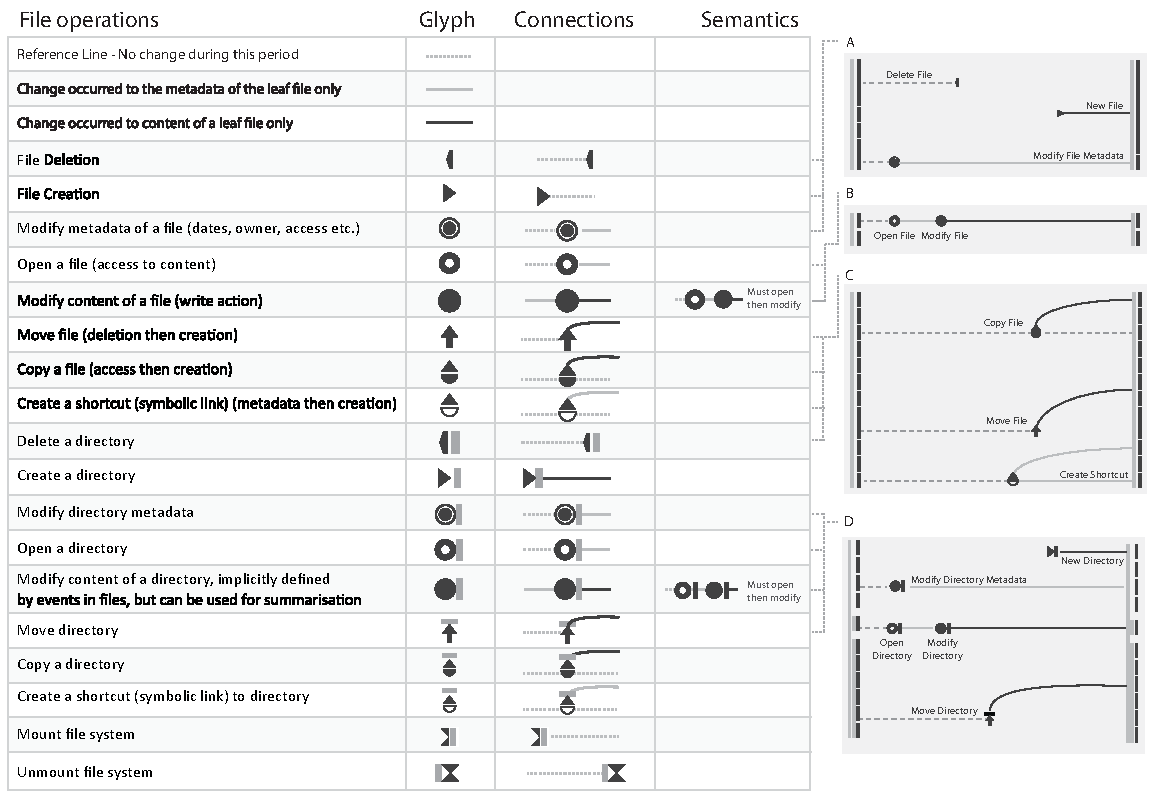
\includegraphics[width=0.99\textwidth]{images/filesystem/table_new}
\end{center}
\caption{Eighteen glyphs designed to represent different events in file systems.
Each event is associated with its primary glyph representation in the second column.
In addition, an event may be associated with special signatures in terms of connection (in the third column) and semantic ordering (in the fourth column).
Semantic ordering refers to how some glyphs will only ever appear in conjunction with another glyph (\eg, modifying a file requires first opening the file \emph{then} modifying its contents).}
\label{table:fileoperations}
\end{figure*}

Differentiability is only one aspect of glyph design.
We have to consider other aspects such as how easy it is to learn and remember glyphs, how glyphs may be connected, and how they may be ordered if the corresponding events happened to the same file or directory?
As shown in Figure~\ref{table:fileoperations}, we utilised similar designs for files and directories to facilitate learning and memorisation.
We also considered how they may be connected.
The three types of connection lines as shown at the top of the Figure~\ref{table:fileoperations} and their different positions (shown in the third column), may add additional features to help differentiate glyphs.
For example, all lines connecting to a \emph{deletion} glyph will always come from the left, and all connecting to a \emph{creation} glyph will extend to the right.
All lines connecting a \emph{copy} or \emph{move} glyph will suggest a spatial shift vertically.
Additionally, semantic ordering, such as \emph{open} before \emph{read}, can make the difference in increasing the QHD of the glyph designs as illustrated on the right side of Figure~\ref{table:fileoperations}.

\subsubsection{Evaluation}
\label{sec:eval_glyphs}

We evaluated those glyphs in Figure~\ref{table:fileoperations} based on the QHD obtained from a human-centric survey and by using computer-based similarity measures.
We used the same survey and metrics as described in Section~\ref{sec:qhd} since this allowed for comparison of the QHD for our glyph set against that of the reference pairs and primitives discussed in Section~\ref{sec:qhd}.
%Note that for our glyphs only the potentially risky pairs were evaluated.

\begin{figure*}[b!]
\begin{center}
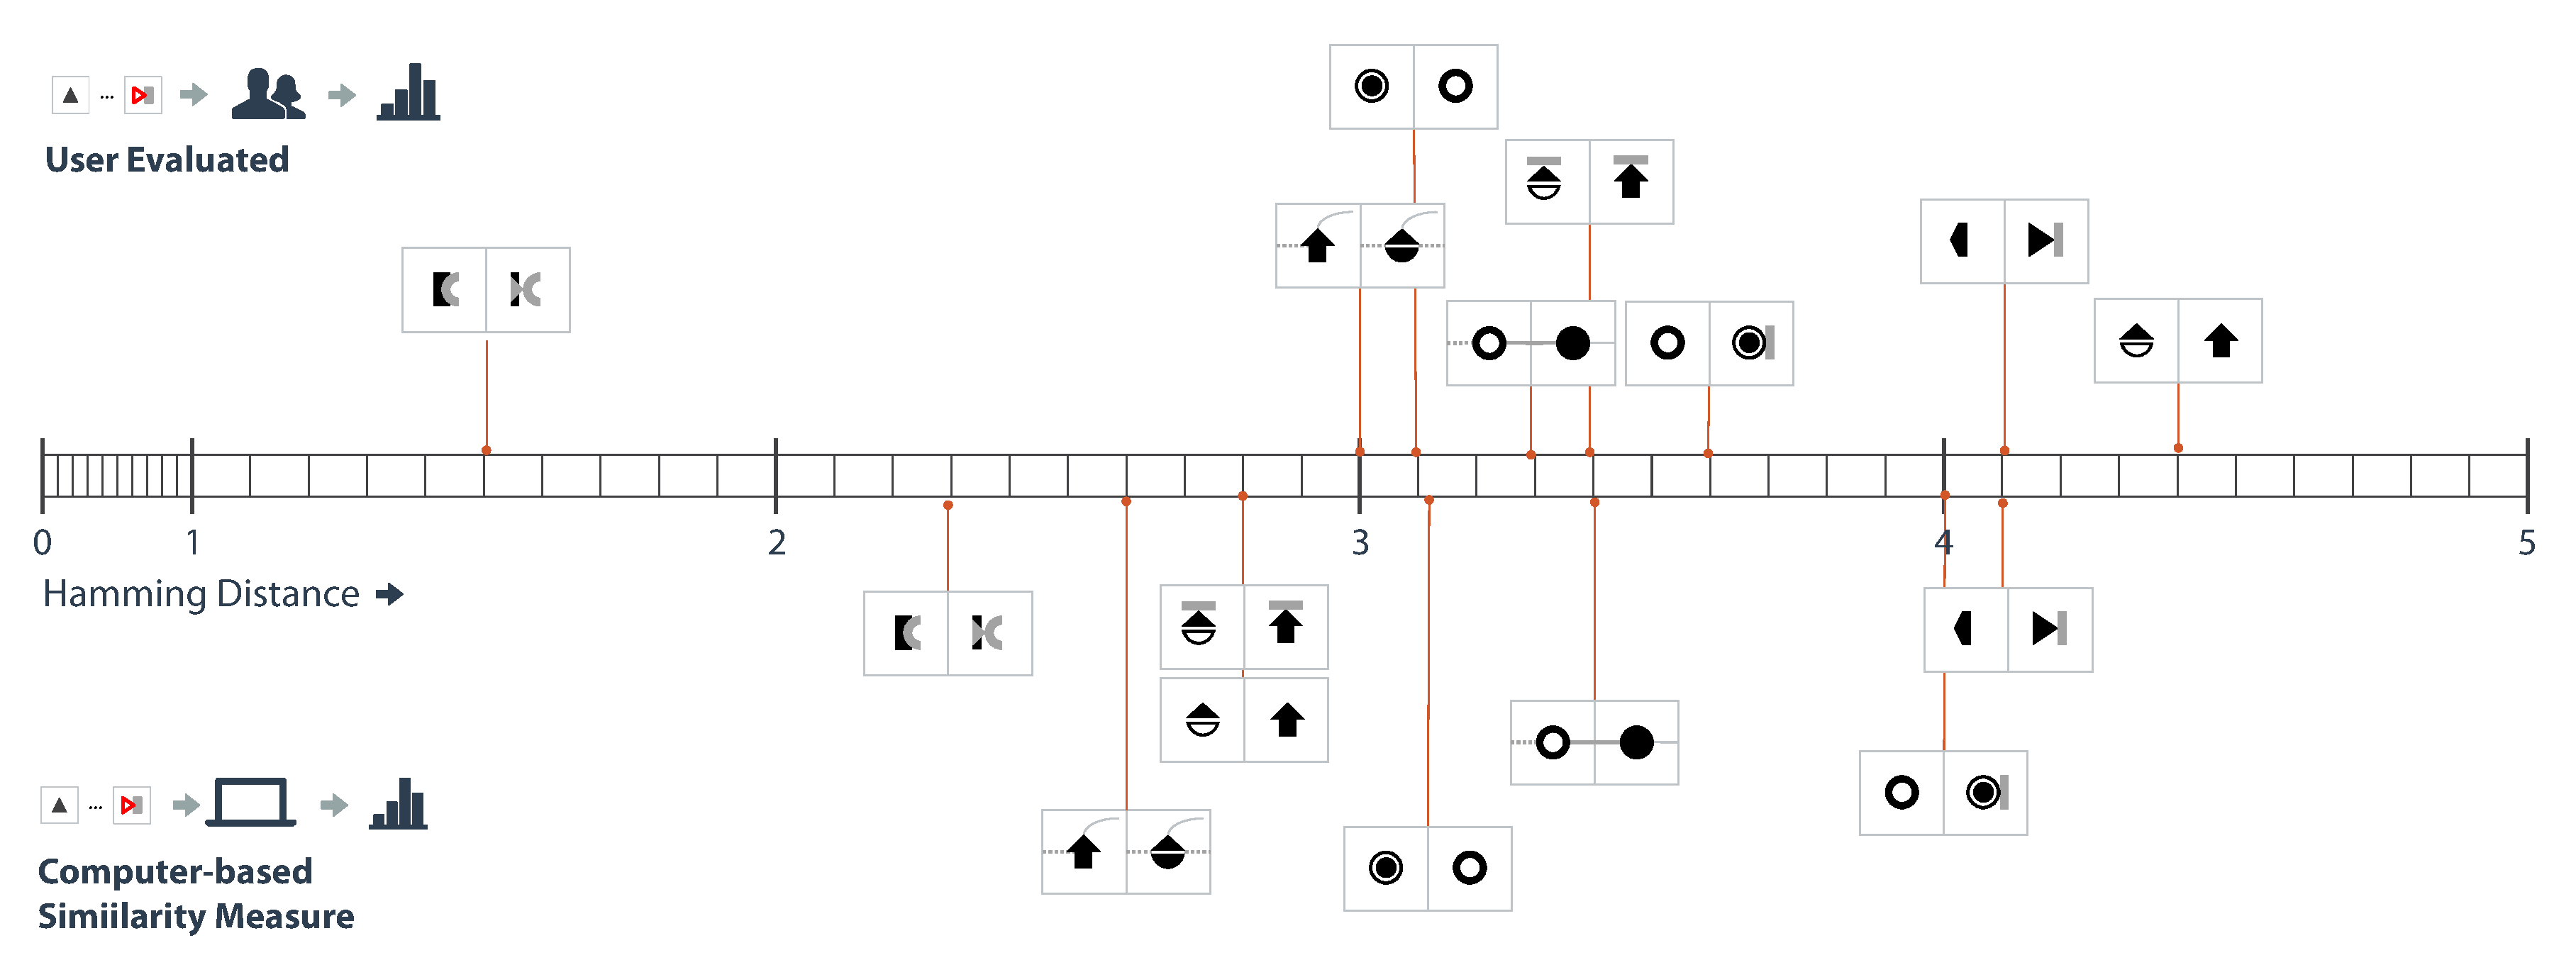
\includegraphics[width=\textwidth]{images/filesystem/Comparison_ourglyphs}
\end{center}
\caption{Sample of results for the file visualization glyph pairs used in both the user-centric estimation (top) and by computer-based similarity measure (bottom).
Low values indicate difficult to differentiate glyphs (bar colour coded in orange/yellow), whilst high values indicate easy to differentiate glyphs (bar colour coded in greens).}
\label{fig:our_glyph_scores}
\end{figure*}


The human-centric estimation provided us with most meaningful insights about the quality of the glyphs.
The 104 pairs of glyphs evaluated by participants have an average QHD of 2.9 bits.
Figure \ref{fig:evaluation_groups} shows the 22 comparison groups used in this evaluation. 
The average QHD for the reference pairs (Groups A and B) is 2.7 bits.
The average for the primitive pairs (Groups C, D, E, F, G, H, I, J) is 2.6 bits.
The average for the potentially risky pairs in our file system glyph set (Groups O, P, Q, R, S, T, U, V, W, X, Y, Z) is 3.2 bits.
Almost all of our glyph pairs have their QHD above 2 bits, except one pair (QHD = 1.5 bits) which was not used in the final design.
The upper part of Figure~\ref{fig:our_glyph_scores} shows a selection of the survey results.

Meanwhile, the computer-based metric also measured our glyph pairs favourably.
The average QHD estimated by the metric is normalised to have the same min, mean and max as the human-centric estimation.
The complete set of 104 glyph pairs have an average QHD of 2.9 bits
The average QHD for the reference pairs is 2.6 bits.
The average for the primitive pairs is 2.7 bits.
The average for the potentially risky pairs in our glyph set is 3.1 bits.
The lowest QHD for our potentially risks glyph pairs is 2.1 bits.


Subsequent research presented by Demiralp \etal in their work on Perceptual Kernels\cite{demiralplearning} further validated our user-based and computer-based results.
Their findings for shape and colour distances are shown in Figure \ref{fig:eval_glyph_scores} A - D.
These results are shown to be consistent with the overall results extrapolated from the user- and computer-based metrics in Figure \ref{fig:eval_glyph_scores} E. 

The evaluation also showed some interesting phenomena.
The additional features added to the directory glyphs have reduced the QHD among directory glyphs.
For example, when comparing Group O and Group Q, where the glyphs for \emph{creation}, \emph{modify metadata}, and \emph{modify content} were compared within the context of files and directories respectively, human-centric estimation shows a noticeable difference.
The average QHD for Group O (files) is 3.4 bits and that for Group Q (directories) is 2.6 bits.
Similarly, for Group T and Group V where \emph{move}, \emph{copy}, and \emph{short cut} glyphs were compared, the average QHD for Group T (files) is 3.3 bits, and that for Group V (directories) is 2.8 bits.
The computer-based similarity measures suggest little difference between O and Q and between T and V.
This indicates a need for further research to better understand the role of integral and separable visual channels.

\subsubsection{Application}
\label{sec:application}

To demonstrate the applicability of the above glyph encoding scheme, we developed an interactive visualization tool for visualising event log data.
In addition to the glyph-based visualization, the system supports a variety of interactions including: file system event filters; user filters; file system navigation; temporal filters; and details on demand;
Here we discuss a use case with Dropbox logs.

\begin{figure*}[ht!]
\begin{center}
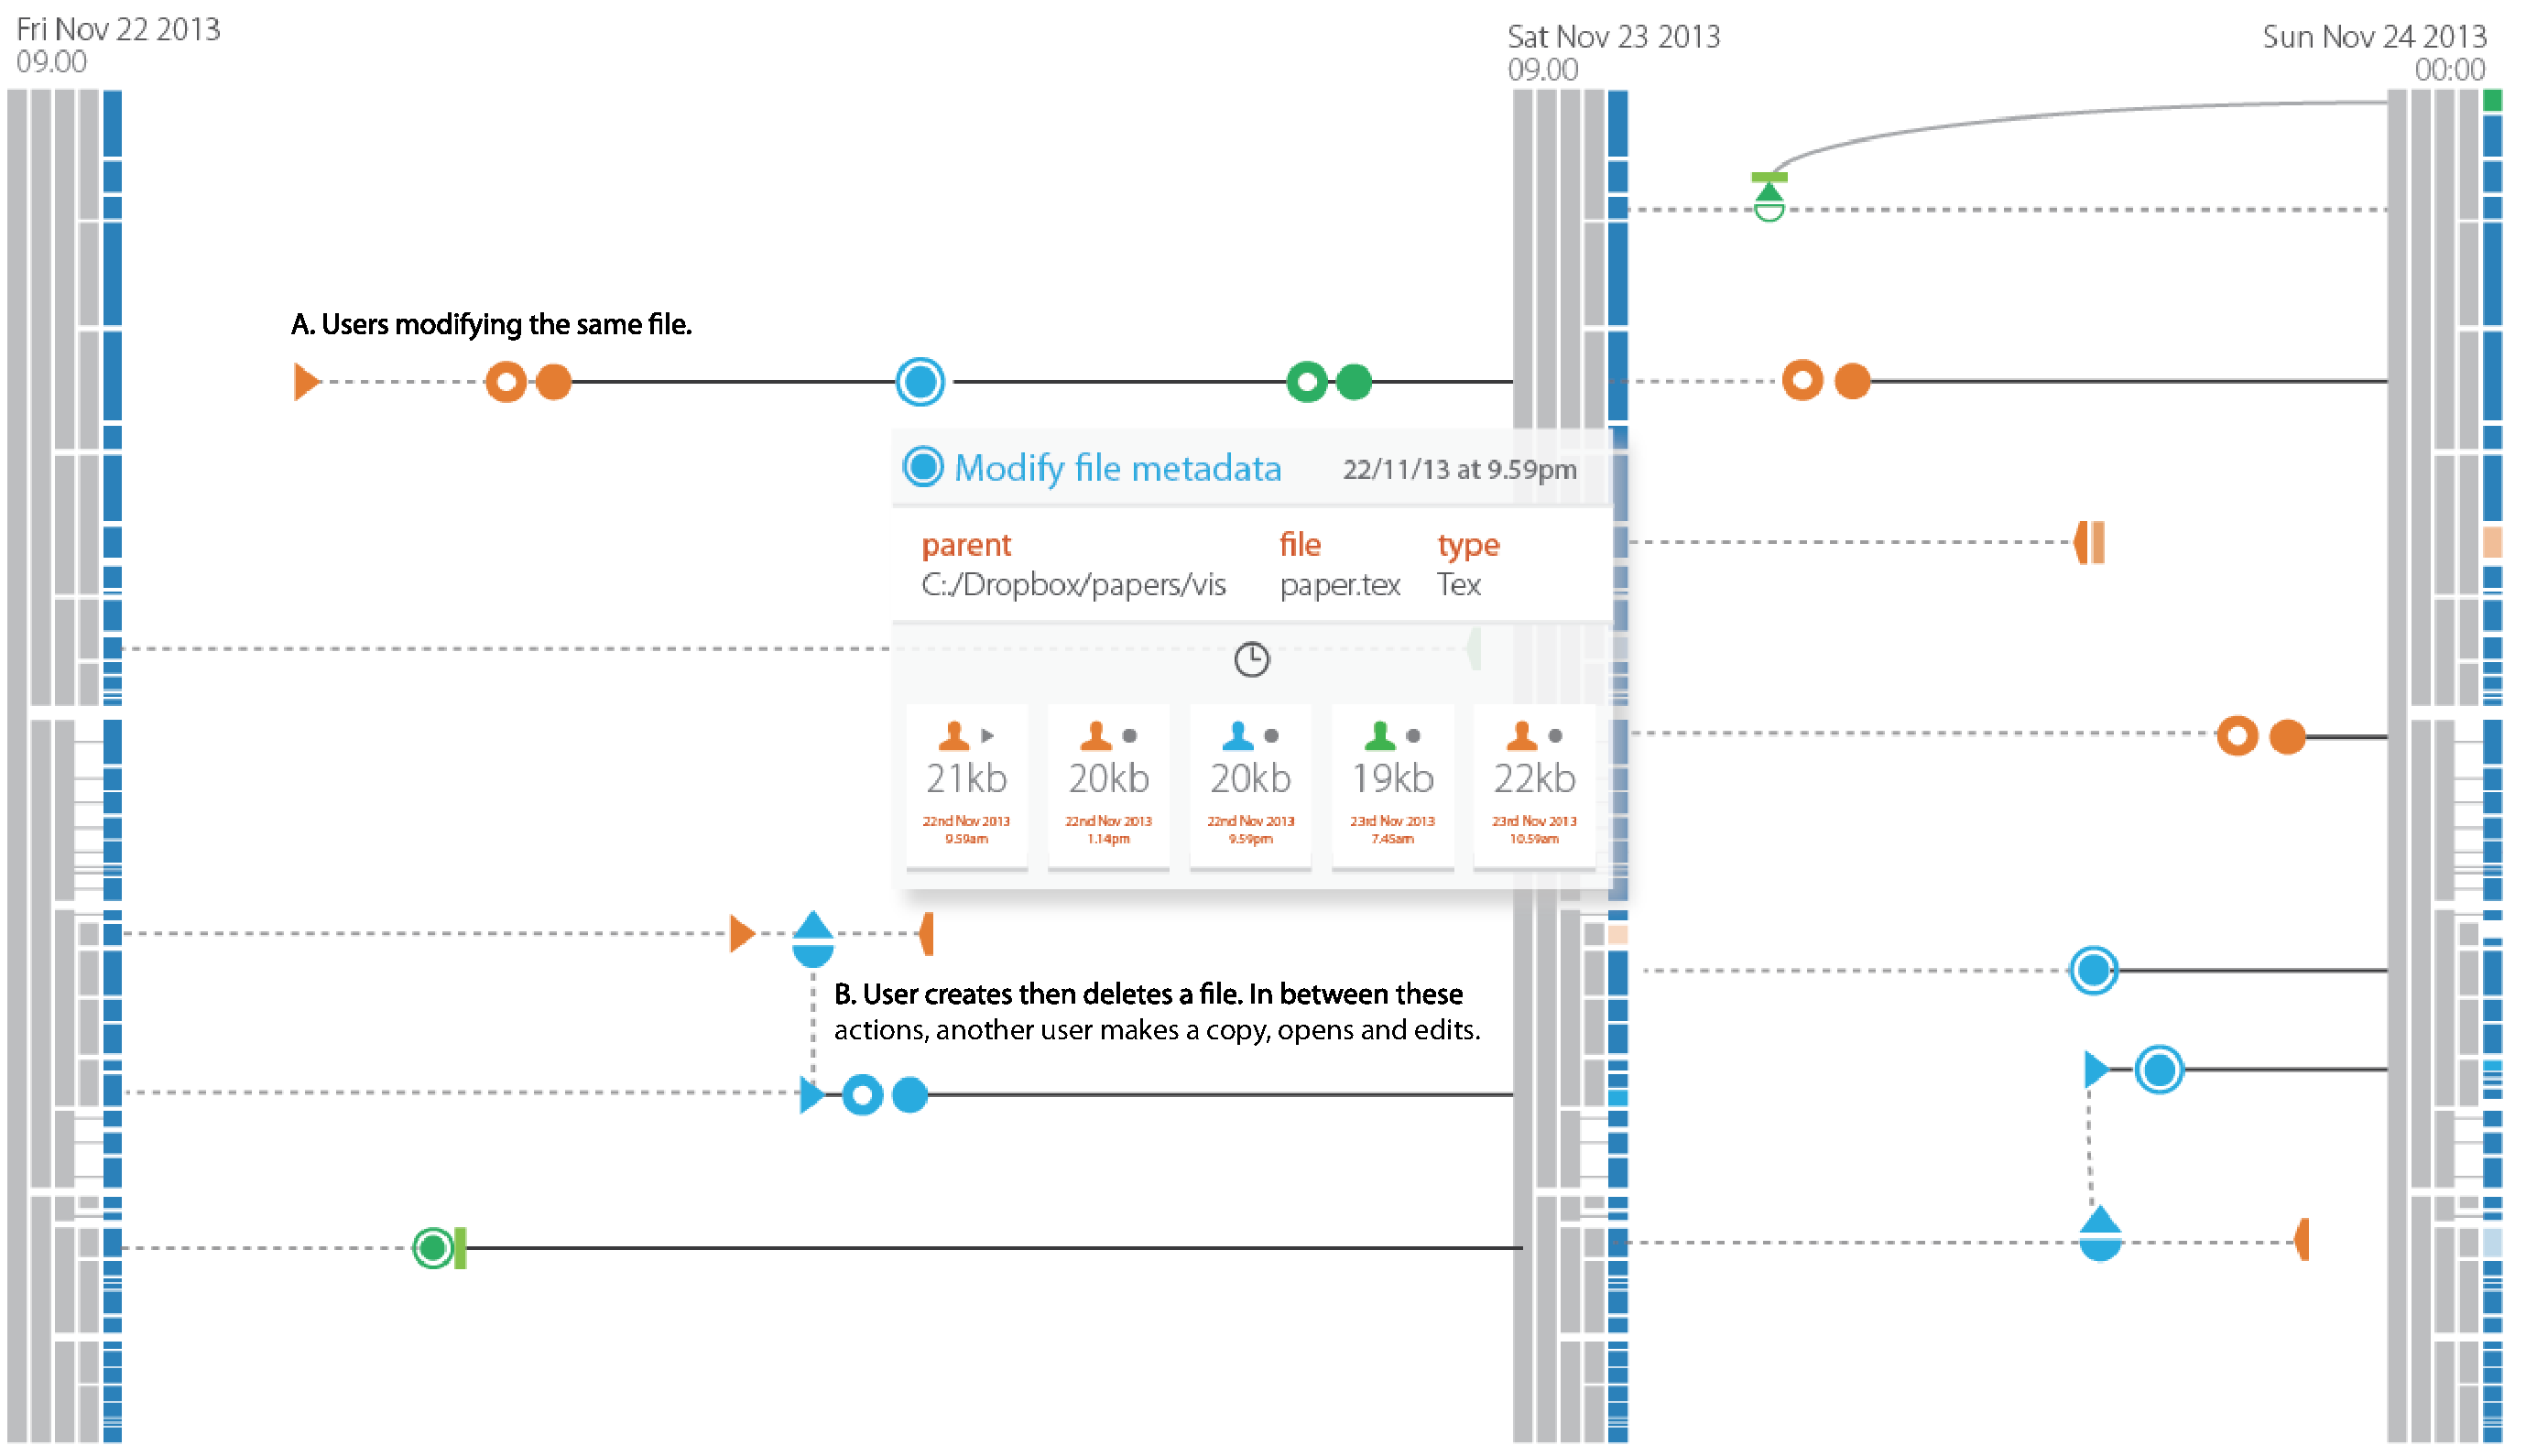
\includegraphics[width=\textwidth]{images/filesystem/dropbox-casestudy-2}
\end{center}
\caption{Glyph-based visualization is used to display events from a Dropbox activity log. The vertical bars are an abstract representation a directory tree and the timeline flows from left to right.
In event A) we can see the case where a number of users have been modifying the same file. The popup gives more details about the modifications, who did them and when. This allows for provenance tracking where such information is available.
In event B) we have another case where \emph{user X} (orange) creates a file, then \emph{user Y} creates a copy of this file, opens it and modifies its contents. \emph{User X} then deletes the original file, however a modified copy exists elsewhere.}
\label{fig:dropbox}
\end{figure*}

%
Dropbox is a popular cloud service that allows users to synchronise their files across multiple devices.
It allows users to create shared directories that other users can be invited to access.
This makes it especially useful for collaborative activities between institutions and colleagues, and for sharing personal media with family and friends.
Therefore it is desirable for users to visualise events in a shared folder, for instance, to see which file has been created or modified recently and by whom.
Although the service does provide a text-based activity log that users can access, it is time-consuming and tedious to read a long list of events.


As shown in Figure~\ref{fig:dropbox}, the glyph-based visualization allows users to gain an overview of the events in a shared folder.
As discussed previously, we avoided the use of colour in the initial glyph design.
This means that the visualization system can use this visual channel to encode additional dimensions, such as users or types of files.
In this example, colour is used to depict different three different users (shown in blue, orange, and green coloured glyphs).

The three vertical bars are simplified views of the directory tree concerned.
The period displayed spans over 39 hours, with a variety of events taking place.
Some indicate close collaboration, when a line of activities linked different users to a single file.
For example, the top line in the left section shows that the orange user created a file, and then opened and modified it.
After several hours, the blue user modified the metadata of the file (possibly renaming it or changing its access date).
Several hours later, the green user opened and modified it.
If a viewer wishes to inspect an event in detail, or simply forget the meaning of a glyph, he/she can simply hover the mouse over the glyph and a pop-up window will display details about the event and the file or directory concerned.
The detailed information includes the filename, the parent directory, and the file type.
It also shows file-specific history, such as the operations that each user performed and the file size after each operation.
Collaborative colleagues can become aware of ongoing actions, reducing the need to inform each other of every file access action via email.

\newpage

\section{Contributions}

This chapter served to show how not all design processes and evaluation techniques need to be the same for systematisation to work.
There will never be a ``one size fits all'' process for glyph design.
The importance of domain specificity and metaphoric representations in glyphs are often key to ensuring their memorability and learnability.
The point of systematisation is to make glyph design more objective (rather than subjective).
This can take on many forms, including structuring how to select the motifs that should be made as glyphs for visual compression, how visual channels should be used in terms of data specificity or natural/semantic mappings, or how glyphs can be composed based on the importance of particular variables in the data?

The three examples in this chapter showed how one or more of the techniques introduced in Chapter \ref{chap:strategies} could be used to inform the design of glyphs.\\


For \textbf{biological sequence visualization}, we have presented a new design for the sequence logo that incorporates glyph-based techniques to aid interpretation.
Our usability tests demonstrated that users generally found consensus sequence reading tasks easier with the new sequence logo.
Users, on the whole, agreed that the new representation did a better job of improving the display of salient information.
The design process did not involve the use of computational approaches.
However the design process was systematised through close domain-expert interaction accompanied by consultation of design principles.
Metaphor was used to decrease the cognitive overhead required to learn new glyph associations.
Evaluation was conducted with an online survey consisting of over forty users who were both familiar and unfamiliar with the sequence logo. 
This work was published as a short paper and presented at EuroVis 2015 in a paper entitled \emph{Redesigning the Sequence Logo with Glyph-based Approaches to Aid Interpretation} \cite{CGF:maguire14-sp}.\\

For \textbf{poetry visualization}, we presented a two-stage approach to:
1) a glyph design to represent the variables of a poem; and
2) an overview glyph to show how sounds change throughout a poem. 

The first piece of work utilised research presented in Chapters \ref{chap:related_work} and \ref{chap:glyph-tax}, which contributed to the overall design (\eg, use of natural mappings).
The design process involved close domain expert interaction to help refine the glyph design.
This is often unavoidable, but it is time consuming.
For example, many of the iterations on the design of the mini-glyph showing how particular sounds are formed could have been removed through computational approaches that could automatically determine which sounds are pronounced within a corpus of English text.
Instead, the 5x7 to 3x3 grid evolution was made possible only through multiple iterations with the domain experts. 
This triggered the idea to experiment with a computational approach for the design of macro glyphs.
This work was published in the Computer Graphics Forum in 2013 in a publication by Abdul-Rahman \etal named \emph{Rule-based Visual Mappings -- with a Case Study on Poetry Visualization} \cite{CGF:Abd2013a}. 

The second piece of work showed how statistical analysis of the data can assist the glyph design process.
Converse to the previous glyph design process, this work partially removed the need for constant domain expert interaction.
Domain experts were only consulted at the start of the design process for requirements elicitation, and at the end for evaluation.
The intermediate stages involved no user interaction.
Through performing statistical analysis of a representative English text collection, we obtained metrics that were able to inform the design process with more precision than was gained from subjective analysis by domain experts.
For example, in the previous work, domain experts took some time to decide which parts of the full 5x7 IPA vowel chart were required to represent sounds in the English language.
From our analyses, this was determined in less than a minute with a representative sample of English text.
Additionally, our analyses also found that two positions from the 3x3 grid were never used in the collection of text we analysed.
The work was evaluated through a semi-structured interview with poetry scholars.
This work was published as a short paper in 2014 in a publication by Abdul-Rahman \etal named \emph{Comparing Three Designs of Macro-Glyphs for Poetry Visualization} \cite{CGF:abdul-rahman14-sp}.\\

For \textbf{file system visualization}, we presented a glyph-based visualization using glyphs whose design was driven by a novel conceptual framework, the \emph{quasi-Hamming distance} (QHD). 
The QHD facilitated a systematic approach to the design of fail-safe glyph encoding schemes.
To demonstrate the feasibility of this conceptual framework, we presented two proof-of-concept experiments, where we obtained QHD measures from a human-centric survey and from computer-based similarity measures.
To demonstrate its practical applicability, we conducted a case study where event logs from Dropbox and Git were visualised using a set of fail-safe glyphs.

This work provides a further stepping stone towards the establishment of a collection of mathematical and cognitive theories, experimental findings and statistics, design techniques and computational metrics for guiding, and aiding glyph design.
However, before the QHD technique is truly useful, two substantial research questions will need to be answered:
1) how can we understand the relationship between the just-noticeable difference measures of various visual channels and the differentiability of glyphs encoded using such visual channels?; and
2) how can we create computer-based metrics, more similar to human-based metrics for determining the distinctiveness of glyphs in a code. 

Nevertheless, this work is a good first step.
Additionally, with work already beginning to surface, \eg, \emph{Perceptual Kernels} \cite{demiralplearning}, the answers to these questions may come sooner rather than later.

